\documentclass[twocolumn]{article}

% ── Author comment macros ────────────────────────────────────────────────────
\newcommand{\red}[1]{{\color{red}#1}}
\newcommand{\todo}[1]{{\color{red}#1}}
\newcommand{\TODO}[1]{\textbf{\color{red}[TODO: #1]}}
\newcommand{\mypar}[1]{\noindent\textbf{#1}}

\newcommand{\anis}[1]{{\color{magenta}{[AR] #1}}}
\newcommand{\einari}[1]{{\color{teal}{[EH] #1}}}
\newcommand{\mete}[1]{{\color{orange}{[MA] #1}}}
\newcommand{\samuli}[1]{{\color{blue}{[SJ] #1}}}

% ── Layout & typography ───────────────────────────────────────────────────────
\usepackage[letterpaper, top=0.75in, bottom=0.75in, left=0.75in, right=0.75in, columnsep=0.25in]{geometry}
\usepackage[protrusion=true,expansion=false]{microtype}

% ── Author affiliations ───────────────────────────────────────────────────────
\usepackage{authblk}
\usepackage{cuted}

% ── Tables ───────────────────────────────────────────────────────────────────
\usepackage{booktabs}
\usepackage{tabularx}
\usepackage{multirow}
\usepackage{adjustbox}

% ── Figures ──────────────────────────────────────────────────────────────────
\usepackage{float}
\usepackage{caption}
\usepackage{subcaption}

% ── References ───────────────────────────────────────────────────────────────
\usepackage{natbib}
\setcitestyle{numbers,square}

% ── Colours & links ──────────────────────────────────────────────────────────
\usepackage[table]{xcolor}
\usepackage[colorlinks=true, linkcolor=blue, urlcolor=cyan, citecolor=green]{hyperref}


\graphicspath{{../figures/}}

\title{\textbf{Host-Conditioned Spatial Structure of Canopy Mortality in Finland's Boreal Forests}}

\author[1]{\textbf{Anis Ur Rahman}}
\author[2,3]{\textbf{Samuli Junttila}}
\affil[1]{CSC -- IT Center for Science Ltd., Espoo, Finland}
\affil[2]{University of Eastern Finland, Joensuu, Finland}
\affil[3]{University of Helsinki, Helsinki, Finland}
\affil[ ]{\texttt{anis.rahman@csc.fi}}

\date{}

\begin{document}

\twocolumn[
  \begin{center}
    \maketitle
    \begin{abstract}
    Finland's boreal forests are experiencing a documented increase in non-harvest tree
    mortality~\citep{junttila2024significant}, and the spatial arrangement of dead trees encodes the
    processes that generate it. We analyse 698,223 individual dead-tree locations (detected by a
    U-Net segmentation model from 2023 aerial imagery across a national-scale sample of seven boreal
    super-sites, $\sim$60.4--67.8\textdegree{}N) as a \emph{host-conditioned point process}, asking
    whether mortality clusters more than forest host availability alone explains. Conditioning on a
    pre-mortality (2021) multi-source forest-inventory host surface, we find that mortality intensity
    increases with both spruce and total growing-stock volume (strong host-tracking), and that,
    beyond this host structure, mortality retains a \emph{modest but genuine residual aggregation}
    that holds from the sub-kilometre scale out to at least 3\,km: the inhomogeneous $L$-function lies
    above a host-conditioned simulation envelope in all seven blocks even under a richer null
    (spruce\,+\,total volume\,+\,stand edge), and the same exceedance appears whether the process is
    taken at the cluster-centroid or the individual-tree level: a local-contagion signature on top of
    host availability that is not an artefact of the clustering unit. We establish these claims with a
    reusable falsification-and-validation harness for morphometrics derived from black-box detection
    models: a covariance-preserving null with mixture-model discreteness diagnostics, clustering
    scale and shape-filter stability gates, detector-confound propagation (cluster ``type''
    predictable from detector confidence alone at AUC\,=\,0.727), and purposive cluster-sample
    inference (effective sample size = 7 blocks, not 14,582 clusters), which also shows that a
    discrete shape-``typology'' of the clusters is an artefact of clustering scale, filter
    thresholds and detector behaviour rather than ecology. We therefore report spatial
    \emph{structure}, not agent-labelled types: lacking species, dating, and ground-truth layers,
    disturbance-agent attribution is withheld. A marked-process test against an external
    disturbance-agent layer is the natural next step.
    \end{abstract}
    \vspace{0.3in}
  \end{center}
]

\textbf{Keywords:} boreal forest mortality; spatial clustering; DBSCAN; Clark--Evans index;
morphological gradient; cluster shape metrics; clustering-scale sensitivity; Finland

% ─────────────────────────────────────────────────────────────────────────────
\section{Introduction}
\label{sec:intro}
% ─────────────────────────────────────────────────────────────────────────────

Boreal forests store roughly 30\% of terrestrial carbon and support exceptional
biodiversity, yet they are undergoing accelerating disturbance as climate change intensifies
drought, windstorms, and pest outbreaks~\citep{bradshaw2015global, allen2010global}.
In Finland, non-harvest tree mortality has increased substantially in recent years
\citep{junttila2024significant}, a trajectory that demands systematic monitoring. Understanding which
ecological processes drive this mortality, and where they concentrate across the
landscape, is a prerequisite for adaptive management and carbon-flux modelling.

The spatial arrangement of dead trees encodes information about the process that killed them.
Bark-beetle outbreaks typically generate dense, spatially contagious patches as infestation
spreads from tree to tree~\citep{raffa2008cross, hlasny2021bark}. Wind damage, by contrast,
tends to produce elongated, directionally oriented swaths aligned with storm tracks
\citep{gardiner2013wind, gregow2011combined}. Drought-induced mortality can produce more
scattered, diffuse patterns tied to soil-water gradients~\citep{mcdowell2008mechanisms}.
These morphological \textit{fingerprints} are in principle recoverable from the spatial arrangement of dead-tree
locations even when individual tree species and cause-of-death records are unavailable.

High-resolution aerial imagery now enables the detection and georeferencing of individual
dead trees over large areas. The 2023 aerial sample used here produced 698,223
dead-tree locations in ETRS89/TM35FIN (EPSG:3067) coordinates, distributed across Finland from the
southern boreal zone to Lapland, a dataset large enough to support robust statistical
characterisation of cluster morphology at scales ranging from the individual stand to the
national sample.

This paper makes three contributions, one empirical and two methodological:
\begin{enumerate}
  \item \textbf{Host-conditioned spatial characterisation of boreal canopy mortality.}
        Treating 698,223 individual dead-tree detections as a point process (their mapped locations
        analysed as a spatial pattern) and conditioning on a pre-mortality forest-inventory host surface, we show that mortality intensity tracks host
        availability (it rises with both spruce and total growing-stock volume) and yet retains a
        modest, genuine \emph{residual aggregation} that survives a richer host-conditioned null
        (spruce\,+\,total volume\,+\,stand edge) from the sub-kilometre scale out to at least 3\,km,
        in all seven blocks and at both the cluster-centroid and individual-tree level: a
        local-contagion signature on top of host-tracking, established with inhomogeneous
        second-order statistics and host-conditioned simulation envelopes.
  \item \textbf{A falsification-and-validation harness for morphometrics from black-box detectors.}
        A reusable, model-agnostic protocol that asks whether spatial statistics computed on
        segmentation outputs reflect ecology or the instrument: a detector-confound test using the
        model's own confidence (cluster ``type'' predictable at AUC\,=\,0.727), detection-error
        propagation through the full pipeline, clustering-scale and shape-filter stability gates, a
        covariance-preserving null with mixture-model discreteness diagnostics, purposive
        cluster-sample inference (effective sample size = the 7 sampling blocks), and an external
        check against forest-inventory species composition. Applied here it
        overturns most candidate signals and certifies the host-conditioned residual.
  \item \textbf{A demonstration that cluster shape alone does not attribute disturbance agent.}
        A candidate two-type morphological ``typology'' of the clusters dissolves under the harness:
        it is not invariant to the clustering radius, its prevalence is an artefact of the
        aspect-ratio filter, and (aspect-ratio-matched) it carries no directional point-process
        signal beyond hull shape; an external check against forest-inventory species composition
        confirms the morphological gradient does not even track the stand species mix. We therefore
        characterise spatial structure rather than infer
        agents from patch geometry, a transferable caution for the aerial mortality-mapping
        literature.
\end{enumerate}

Throughout, we deliberately withhold disturbance-agent labels. Morphological associations with
wind, bark beetle, or other agents are testable hypotheses, not findings: confirmed attribution
would require species records, mortality dates linked to known events (the available
\texttt{alku\_aika} field records flight-strip acquisition time, not mortality date), and
multi-temporal imagery, none of which are present in the current dataset. We return to specific
attribution caveats, including the absence of any directional signal in the elongated type, in
the Discussion.

% ─────────────────────────────────────────────────────────────────────────────
\section{Related Work}
\label{sec:related}
% ─────────────────────────────────────────────────────────────────────────────

\mypar{European forest disturbance ecology and mapping.}
Europe's forests have been subject to intensifying disturbance regimes over recent decades,
driven by the interaction of climate change with biotic and abiotic agents
\citep{seidl2011unraveling, seidl2017forest}. \citet{senf2021mapping} produced the first
continent-wide map of forest disturbance regimes using satellite time series, revealing
strong latitudinal gradients in the relative importance of wind, bark beetles, and fire.
\citet{allen2010global} documented globally the accelerating role of drought and heat as
pre-disposing stressors that increase forest vulnerability to secondary agents. These
landscape-scale perspectives highlight the need for methods that can characterise disturbance
not just by area affected, but by the spatial structure of affected patches.

\mypar{Bark beetle ecology and spatial signatures.}
The Eurasian spruce bark beetle (\textit{Ips typographus}) is the dominant biotic disturbance
agent in boreal and subalpine Europe~\citep{hlasny2021bark}. \citet{raffa2008cross} showed
that bark-beetle eruptions are governed by cross-scale feedbacks: fine-scale tree-to-tree
contagion at the stand level, mediated by pheromone plumes and resource depletion, scales up
to landscape-level epidemics when predisposing conditions (drought, windthrow) are met.
\citet{jonsson2012epidemics} analysed epidemic dynamics of \textit{Ips typographus} in
Sweden, identifying that outbreaks initiated in windthrown timber and then spread as
self-reinforcing patch growth. \citet{kautz2011simulating} demonstrated that high-resolution
empirical host-tree distributions can be used to simulate outbreak spread, predicting the
compact, dense patch morphology that characterises beetle kills. \citet{wichmann2001spread}
documented how storm-felled timber from the 1999 Danish windstorm acted as a beetle
breeding reservoir, amplifying subsequent outbreaks and leaving spatially contagious kill
patches.

\mypar{Wind damage in Fennoscandia.}
Wind is the leading abiotic disturbance agent in northern European forests
\citep{schelhaas2003natural}. \citet{gardiner2013wind} reviewed how silvicultural history,
stand structure, and edge exposure interact to determine windstorm susceptibility, noting that
clearcut edges and monoculture Norway spruce stands are particularly vulnerable.
\citet{gregow2011combined} specifically modelled combined wind and snow-loading risks in
Finland under current and projected future climate, finding that snow-induced stem damage
concentrated in central and eastern Finland may increase with warming winters. The elongated,
directional morphology of wind-felled areas has been noted in several Fennoscandian studies
as a diagnostic feature distinguishing wind damage from beetle-induced mortality.

\mypar{Spatial statistics methods.}
The Clark--Evans statistic~\citep{clarkevans1954} remains the canonical index of point
dispersion within bounded study regions. \citet{donnelly1978} derived an analytical edge
correction that removes the downward bias introduced by boundary effects in finite study
areas, making the corrected statistic suitable for small clusters with irregular convex-hull
boundaries. \citet{anselin1995local} introduced Local Indicators of Spatial Association
(LISA), enabling the identification of statistically significant spatial clusters and outliers
at multiple scales. \citet{wiegand2014handbook} provide a comprehensive treatment of
spatial point-pattern analysis methods for ecological applications, including the mark
correlation function, Ripley's $K$, and related second-order statistics that complement
the first-order metrics used here.

% ─────────────────────────────────────────────────────────────────────────────
\section{Methods}
\label{sec:methods}
% ─────────────────────────────────────────────────────────────────────────────

\subsection{Dataset}
\label{sec:data}

The dataset comprises 698,223 dead-tree locations produced internally by applying the
individual-tree mortality U-Net segmentation model of \citet{junttila2024significant} to
high-resolution aerial imagery acquired in 2023; the underlying detection dataset is not yet
publicly released. The detections come from 312 aerial
image tiles distributed across Finland, spanning roughly 60.4--67.8\textdegree{}N and
21.6--29.6\textdegree{}E, from the southern boreal zone to Lapland, in discrete latitudinal
bands rather than continuous wall-to-wall coverage. Coordinates are provided in ETRS89/TM35FIN
(EPSG:3067), a conformal transverse Mercator projection with metric units, appropriate for
distance-based spatial analyses. The dataset is therefore a \emph{national-scale but spatially
discontinuous sample}: reported cluster prevalences and densities are sample statistics across the
surveyed tiles and should not be read as an exhaustive national census. Figure~\ref{fig:sampling}
shows the sampling footprint, discrete study blocks from the southern coast to Lapland.

\begin{figure}[!htb]
  \centering
  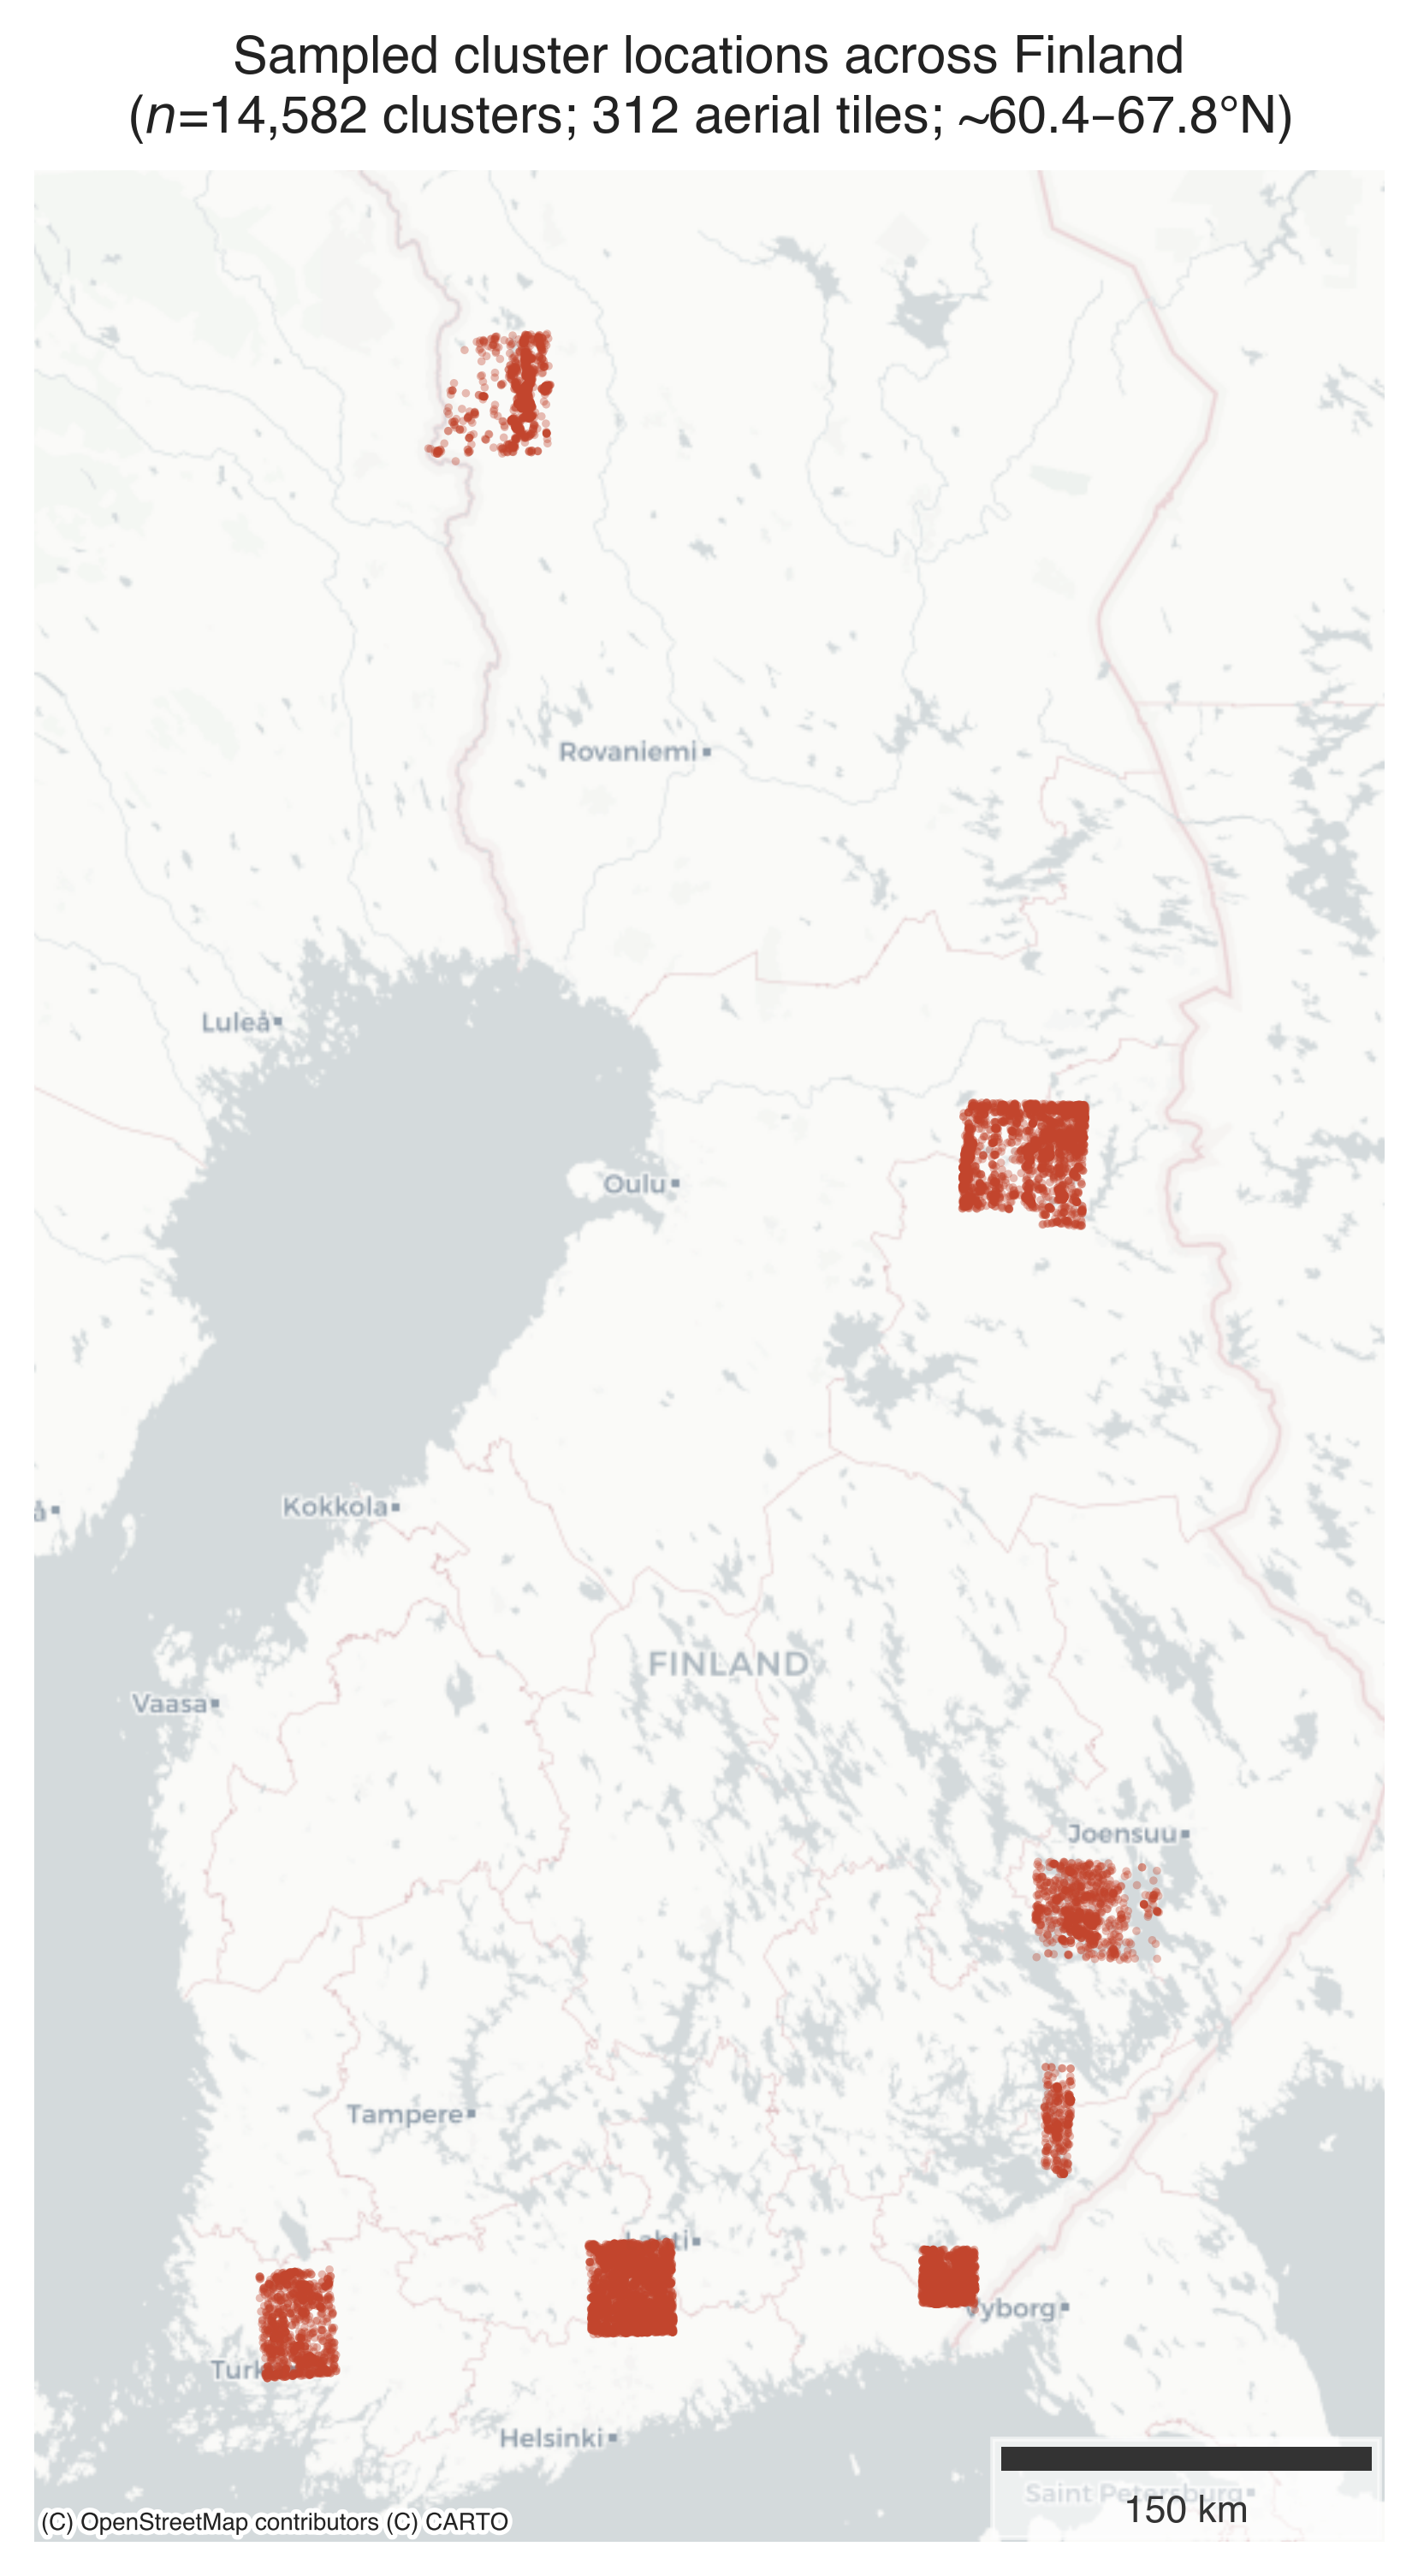
\includegraphics[width=0.7\linewidth]{fig_sampling_extent.png}
  \caption{Sampling footprint: all 14,582 cluster centroids (from 312 aerial tiles) on a national
           basemap. The tiles form discrete study blocks spanning $\sim$60.4--67.8\textdegree{}N
           (southern boreal zone to Lapland) and the full longitudinal width, rather than
           contiguous national coverage.}
  \label{fig:sampling}
\end{figure}

\mypar{Sampling design.}
Formally the data constitute a \emph{purposive two-stage cluster sample}, not a probability sample
of Finnish forest and not a national census. The primary units are 7 spatially contiguous blocks
(``super-sites''), each a mosaic of adjacent 6\,km tiles spanning 25--54\,km and separated from its
neighbours by 84--348\,km (median 149\,km); the secondary units are the 6\,km map-sheet tiles; and
within each tile all detectable dead-tree canopies are enumerated (a within-tile census). The
blocks were compiled operationally rather than drawn under a known probability mechanism, so
design-based inference to a national population is not available and we adopt a model-based,
block-conditional stance throughout. Crucially, the 14,582 clusters are not independent draws: they
are nested within 7 blocks that share imagery campaign, climate band, host composition, and
detector behaviour, so the effective sample size for any between-block or national statement is
governed by the number of blocks (7), not the number of clusters. We therefore restrict inferential
claims to within-cluster and within-block morphology, report prevalences as conditional on the
sampled blocks (and on the eps and AR choices; Section~\ref{sec:res-sensitivity}), and treat the
phrase ``national-scale'' as describing the latitudinal \emph{extent} of the sample, never national
coverage or national population estimates.

\subsection{Clustering}
\label{sec:clustering}

Density-based spatial clustering was performed using DBSCAN~\citep{ester1996density} with
neighbourhood radius eps\,=\,20\,m and minimum neighbourhood size min\_samples\,=\,3.
The eps\,=\,20\,m threshold was chosen to capture within-stand tree-to-tree spread typical
of both bark-beetle and wind disturbance, while separating clusters arising from distinct
events. The 43,539 raw clusters were post-filtered to retain only those satisfying:
\begin{itemize}
  \item $n \geq 5$ trees (excludes trivially small groups),
  \item area $\geq 100$\,m$^2$ (minimum ecologically meaningful patch size),
  \item aspect ratio $\leq 10$ (removes linear artefacts such as road corridors).
\end{itemize}
This yielded 14,582 clusters for analysis.

\subsection{Spatial Metrics}
\label{sec:metrics}

Each cluster was characterised by the following spatial metrics.

\mypar{Within-cluster nearest-neighbour distance (NND).}
For a cluster containing $n$ points, the NND for point $i$ is
\begin{equation}
  d_i = \min_{j \neq i} \| \mathbf{p}_i - \mathbf{p}_j \|,
\end{equation}
and the cluster-level summary statistics are $\overline{\mathrm{NND}} = n^{-1}\sum_i d_i$
and $\sigma_{\mathrm{NND}} = \sqrt{n^{-1}\sum_i (d_i - \overline{\mathrm{NND}})^2}$.

\mypar{Clark--Evans index with Donnelly edge correction.}
The Clark--Evans index compares the observed mean NND to its expectation under complete
spatial randomness~\citep{clarkevans1954}:
\begin{equation}
  R = \frac{\overline{\mathrm{NND}}}{E[\bar{r}]},
\end{equation}
where $R < 1$ indicates clustering and $R > 1$ indicates dispersion.
For small, bounded clusters the uncorrected expectation $E[\bar{r}] = 0.5\sqrt{A/n}$
is negatively biased by boundary effects. Following \citet{donnelly1978}, we use the
corrected expectation
\begin{equation}
  E[\bar{r}] = 0.5\sqrt{\frac{A}{n}}
              + \left(0.0514 + \frac{0.041}{\sqrt{n}}\right)\frac{P}{n},
  \label{eq:donnelly}
\end{equation}
where $A$ is the convex-hull area of the cluster and $P$ is its perimeter.

\mypar{Fractal dimension.}
Boundary complexity is quantified by the box-counting fractal dimension:
\begin{equation}
  D = -\lim_{\epsilon \to 0}
      \frac{\log N(\epsilon)}{\log \epsilon},
\end{equation}
where $N(\epsilon)$ is the number of boxes of side length $\epsilon$ that intersect the
cluster's convex hull. In practice $D$ is estimated as the slope of
$\log N(\epsilon)$ versus $\log(1/\epsilon)$ over a range of scales expressed as fractions of
the hull's bounding-box diagonal. Because the metric is computed on the convex hull rather than
the raw point set, it measures the area-filling complexity of the hull boundary; for the small
clusters that dominate the dataset (median eight points) it is correspondingly coarse, and we
treat it as a descriptive shape index rather than a true fractal estimate.

\mypar{Compactness (form factor).}
\begin{equation}
  C = \frac{4\pi A}{P^2},
\end{equation}
where $A$ and $P$ are the convex-hull area and perimeter. $C = 1$ for a circle and
decreases as the shape becomes more elongated or irregular.

\mypar{Aspect ratio.}
The aspect ratio is the ratio of the major to minor axis of the minimum-area bounding
rectangle:
\begin{equation}
  \mathrm{AR} = \frac{\ell_{\max}}{\ell_{\min}}.
\end{equation}

\mypar{Alpha compactness.}
\begin{equation}
  \mathrm{AC} = \frac{\mathrm{area}(\mathcal{A}_\alpha)}{\mathrm{area}(\mathcal{H})},
\end{equation}
where $\mathcal{A}_\alpha$ is the alpha shape of the point set and $\mathcal{H}$ is its
convex hull. Values near 1 indicate dense, convex clusters; lower values indicate
concave or elongated clusters with interior voids.

\mypar{Core-to-edge ratio.}
The ratio of the convex hull's interior area to its total area, where the interior is the hull
eroded inward by a fixed 1\,m buffer: $\mathrm{area}(\mathcal{H} \ominus 1\,\mathrm{m})/\mathrm{area}(\mathcal{H})$.
Because the erosion width is fixed while clusters vary in size, this ratio is partly a proxy for
absolute cluster size (small clusters lose proportionally more area), which should be borne in
mind when interpreting it.

\mypar{Orientation.}
PCA is applied to the $xy$ coordinates of cluster points; the orientation angle is
\begin{equation}
  \theta = \arctan\!\left(\frac{v_y}{v_x}\right),
\end{equation}
where $\mathbf{v} = (v_x, v_y)$ is the first principal eigenvector. $\theta$ is folded
into $[0^\circ, 180^\circ)$ for use as axial data in orientation analysis.

\subsection{Morphological Gradient and Candidate Partition}
\label{sec:typology}

K-means clustering was applied to the standardised feature vector
(fractal\_dim, clark\_evans, aspect\_ratio) using $k \in \{2, \ldots, 7\}$.
The optimal $k$ was selected by jointly evaluating the silhouette coefficient,
Calinski--Harabasz (CH) score, and Davies--Bouldin (DB) index. At $k=2$ these were
silhouette\,=\,0.401, CH\,=\,8767, DB\,=\,1.073, the best combined performance
across the tested range.

To assess whether the observed silhouette score reflects genuine structure rather than the
covariance of correlated marginals, we compared it against a \emph{covariance-preserving} null:
999 surrogate datasets were drawn from a single multivariate Gaussian whose mean and full
covariance matrix match the standardised feature matrix, and $k=2$ K-means was refitted to each.
This is a stricter null than independent column-shuffling (which destroys all inter-feature
correlation and is therefore beaten by any correlated data); it asks specifically whether the
data are \emph{more clustered than a single elongated Gaussian cloud}. The observed silhouette
(0.401) exceeded the null mean (0.321) and 95th percentile (0.324), giving $p = 0.001$.

Because a significant silhouette does not by itself establish that two discrete classes exist,
we additionally tested for discreteness. Gaussian-mixture model selection by BIC over
$k \in \{1,\ldots,7\}$ and the modality of the first principal component (which captures 60\%
of feature variance) jointly indicate that the morphological features form a continuous
gradient rather than two separated modes (Section~\ref{sec:res-typology}). We therefore treat
the $k=2$ partition as an interpretive summary of the dominant compactness--elongation axis, not
as evidence of a natural class boundary.

\subsection{Orientation Analysis}
\label{sec:orientation}

Cluster orientations $\theta \in [0^\circ, 180^\circ)$ are axial data and must be doubled before
applying circular statistics~\citep{wiegand2014handbook}. The Rayleigh test for uniformity
was applied to the doubled angles $2\theta \in [0^\circ, 360^\circ)$ using pycircstat.
The mean resultant length $r = \|\sum \exp(i \cdot 2\theta_j)\| / n$ and its associated
$p$-value quantify whether orientations depart from a uniform (no preferred direction)
distribution. Results were stratified by type.

\subsection{Spatial Autocorrelation}
\label{sec:morans}

Global Moran's $I$ was computed for four cluster-level metrics
(fractal\_dim, clark\_evans, aspect\_ratio, compactness) at five spatial thresholds
(200, 500, 1000, 2000, 5000\,m) using a random subsample of $n=2{,}000$ clusters stratified by
block, which preserves the regional structure while keeping the dense distance-band weight matrix
tractable. A distance-band contiguity at threshold $\delta$ ($d_{ij} \leq \delta$) was used, with the
weights row-standardised ($\sum_j w_{ij} = 1$). With 20 simultaneous tests we applied a
Bonferroni-corrected significance threshold $\alpha^* = 0.05/20 = 0.0025$; significance is
assessed with the analytical (normal-approximation) $p$-value, since a 999-permutation $p_{\rm sim}$
floor of $10^{-3}$ is the coarsest resolution that can reach $\alpha^*$ and a 199-permutation
test (floor $5\times10^{-3}$) cannot. To test whether any autocorrelation is an artefact of
upstream detection error rather than ecology, we additionally propagated a 15\% random
false-negative detection perturbation through the metric computation over 100 realizations and
recorded the fraction preserving the sign and Bonferroni significance of $I$ at each
metric$\,\times\,$threshold (a detection-robustness gate). Because the sample comprises discrete
latitudinal bands separated by large gaps, the distance-band weights connect only within-band
neighbours at all thresholds tested; the resulting statistic is therefore an estimate of
\emph{within-band} autocorrelation, and we report per-threshold neighbour counts to expose how
thin the short-distance support is.

Local Moran's $I$ (LISA; \citealt{anselin1995local}) was computed to identify
statistically significant spatial clusters (high--high and low--low) and spatial
outliers in fractal dimension.

\subsection{Landscape Connectivity}
\label{sec:connectivity}

A proximity graph was constructed by connecting all cluster centroids within 200\,m
\citep{urban2001landscape}. The reach of a cluster is defined as the number of other
clusters reachable within the connected component to which it belongs. Betweenness
centrality was computed to identify bridge clusters whose removal would fragment the
network. Reach distributions were compared between types using the Mann--Whitney $U$ test.

\subsection{Held-Out Classifier}
\label{sec:classifier}

To test whether the $k=2$ partition is recoverable in a feature space not used to define it,
we trained a Random Forest classifier using only features \textit{not} input to K-means:
compactness, alpha\_compactness, core\_to\_edge\_ratio, nnd\_mean, nnd\_std,
orientation, and reach\_200m. (We note that \texttt{orientation} is axial data on
$[0^\circ,180^\circ)$ entered here as a linear feature, so the tree splits cannot exploit its
circular structure; given its low importance below, this does not affect the conclusions.)
Spatial block cross-validation (GroupKFold, 5 folds,
$100 \times 100$\,km grid, 12 blocks, mean 1215 clusters/block) was used to prevent
spatial leakage. We caution that the blocks are size-imbalanced, the five largest hold roughly
four-fifths of the clusters, so the tight fold-to-fold AUC range understates true spatial
variability. SHAP values~\citep{lundberg2017unified} were computed to assess feature importance.

\subsection{Stability Gates}
\label{sec:sensitivity}

These gates are deliberate attempts to \emph{falsify} our own two-type result: a genuine ecological
partition should survive them, whereas one manufactured by an analysis choice should break. To test
whether the $k=2$ partition is a genuine structure or an artefact of the pipeline's free parameters,
we re-ran the entire pipeline from the raw points under four gates.

\mypar{(G1) Scale stability.}
We re-clustered the raw points at eps $\in \{10,15,20,25,30,40\}$\,m and, at each scale, recomputed
all shape metrics, re-applied the filters, and re-fitted $k=2$ K-means. A genuine class should be
eps-invariant in prevalence and in its feature-space centroid; an artefact of detection chaining
rescales with eps.

\mypar{(G2) Aspect-ratio filter, from raw.}
The AR\,$\leq 10$ filter is applied to the very axis on which K-means clusters, so it cannot be
tested on the already-filtered table. We instead recomputed metrics on all clusters at eps\,=\,20\,m
with \emph{no} AR cap, then applied caps $\in \{5,7,10,15,20,\infty\}$, re-fitting K-means at each and
tracking type prevalence, the within-Type\,0 AR distribution, and the adjusted Rand index (ARI) of
membership against the AR\,$\leq 10$ partition.

\mypar{(G3) Directional second-order structure.}
Hull aspect ratio is a first-order summary and cannot distinguish a linear (wind-swath) point
arrangement from an elongated but space-filling patch. For each cluster we computed the point-scatter
linearity $\ell = \lambda_1/(\lambda_1+\lambda_2)$ from the PCA eigenvalues and a pairwise-displacement
axial resultant, and compared Type\,0 against Type\,1 \emph{within matched hull-AR bins}.

\mypar{(G4) Detection confound.}
The upstream detector provides a per-detection confidence (\texttt{max\_value}) not otherwise used.
We tested whether per-cluster detection covariates (mean/SD confidence, $n$, density) predict type
(5-fold logistic AUC), and whether modest false-negative perturbation (dropping 10--20\% of detections
per cluster and re-fitting) changes type assignments.

\mypar{(G5) External species validation.}
To break the circularity of reading an agent off the shape we clustered on, we attached an external,
non-shape variable to each cluster: the pre-mortality (2021) MS-NFI growing-stock volume of spruce,
pine and birch, sampled at the cluster centroid (EPSG:3067, nodata-masked; clusters off forest host
dropped). We then asked whether the morphological gradient tracks the species mix of the stand that
died, with the block as the replicate: a within-block Spearman correlation between aspect ratio and
each species fraction combined across the seven blocks by a sign test, and a per-block comparison of
species fractions between the two morphological endpoints. No per-cluster $p$-value is reported (it
would be pseudo-replicated across $\sim$2{,}000 clusters per block).

\subsection{Host-Conditioned Point-Process Analysis}
\label{sec:methods-host}

To ask whether mortality clusters \emph{more than forest host availability alone predicts}, we
replace the homogeneous-CSR null, meaningless over heterogeneous forest, with an
\emph{inhomogeneous} null whose first-order intensity is driven by host. In plain terms, the baseline
we compare against is not ``dead trees scattered evenly across the landscape'' but ``dead trees in
proportion to how much host forest is present''; any clustering beyond that baseline (what we call
\emph{residual aggregation}) is the part not explained by where the forest is. The host surface is the
Multi-Source National Forest Inventory (MS-NFI) spruce growing-stock volume from \emph{2021}, i.e.\
\emph{before} the 2023 mortality: a 2023 host layer would be endogenous, since dead spruce drops out
of the standing-volume estimate. The observation window is the union of the 6\,km map-sheet tiles
restricted to forest land (MS-NFI land-class mask), not the tile bounding boxes (which include
lakes) and not ``spruce $>0$'' (which would conflate covariate and window). We model the intensity
$\lambda(u)$ by a pixel-Poisson log-linear fit on the forest grid (covariates: spruce volume, total
growing-stock volume, distance to stand edge) and assess second-order structure with the
inhomogeneous $K$- and $L$-functions and pair-correlation, pooled across tiles with translation edge
correction. Significance is by \emph{host-conditioned} simulation envelopes (99 realisations from the
fitted inhomogeneous null), not the CSR contrast. The estimator was validated on simulated
inhomogeneous-Poisson patterns ($L_{\rm inhom}\!-\!r\approx0$). We run two independent
implementations: a tile-pooled inhomogeneous pair-correlation/$L$ (intensity normalised per tile;
the ring estimator on 6\,km tiles is reliable to $r\lesssim1$\,km, $\approx$ window/4), and a
per-block $L_{\rm inhom}$ in \texttt{spatstat} with the intensity fitted globally (pooled Poisson
across forest cells), cumulative translation-corrected and therefore variance-stabilised, on the
25--54\,km block windows, which extends the reliable range to $r\le3$\,km. Both are run on cluster
centroids and, for the \texttt{spatstat} leg, also on the individual dead trees (intensity fitted on
per-cell tree counts; the point pattern uniformly subsampled to $\le$20{,}000 per block with the null
intensity rescaled to the observed count), so the result does not depend on the analysis unit.

% ─────────────────────────────────────────────────────────────────────────────
\section{Results}
\label{sec:results}
% ─────────────────────────────────────────────────────────────────────────────

\subsection{Cluster Characterisation}
\label{sec:res-char}

The 14,582 filtered clusters span a broad range of sizes and morphologies
(Figure~\ref{fig:histograms}). The median cluster contains 8 trees
(mean\,=\,13.75, SD\,=\,44.03, max\,=\,2{,}965), reflecting a highly right-skewed
size distribution dominated by small clusters but with a heavy tail of large events.
Median area is 388\,m$^2$ (mean\,=\,1{,}061\,m$^2$, SD\,=\,5{,}003\,m$^2$).
Shapes are moderately compact (mean compactness\,=\,0.595, SD\,=\,0.143,
median\,=\,0.609) and moderately elongated (mean AR\,=\,2.548, SD\,=\,1.357,
median\,=\,2.211). The Donnelly-corrected Clark--Evans index (mean\,=\,1.766,
SD\,=\,0.393, median\,=\,1.753) is greater than unity, nominally indicating
more-regular-than-Poisson spacing. We read this cautiously: at a median of eight points per
cluster the index is high-variance, and DBSCAN's minimum-density requirement (min\_samples within
eps) imposes a spacing floor that mechanically inflates apparent regularity, so the value should
not be over-interpreted as an ecological property of tree placement. Mean within-cluster NND is
7.79\,m (SD\,=\,2.43\,m), consistent with individual-tree-scale spacing. Fractal dimension
averages 1.650 (SD\,=\,0.077).

Correlation analysis (Supplementary Fig.~S1) shows strong positive covariation
among size metrics ($n$, area) and expected trade-offs between compactness and aspect
ratio. Supplementary Fig.~S2 presents key pairwise scatter plots.

\begin{figure}[!htb]
  \centering
  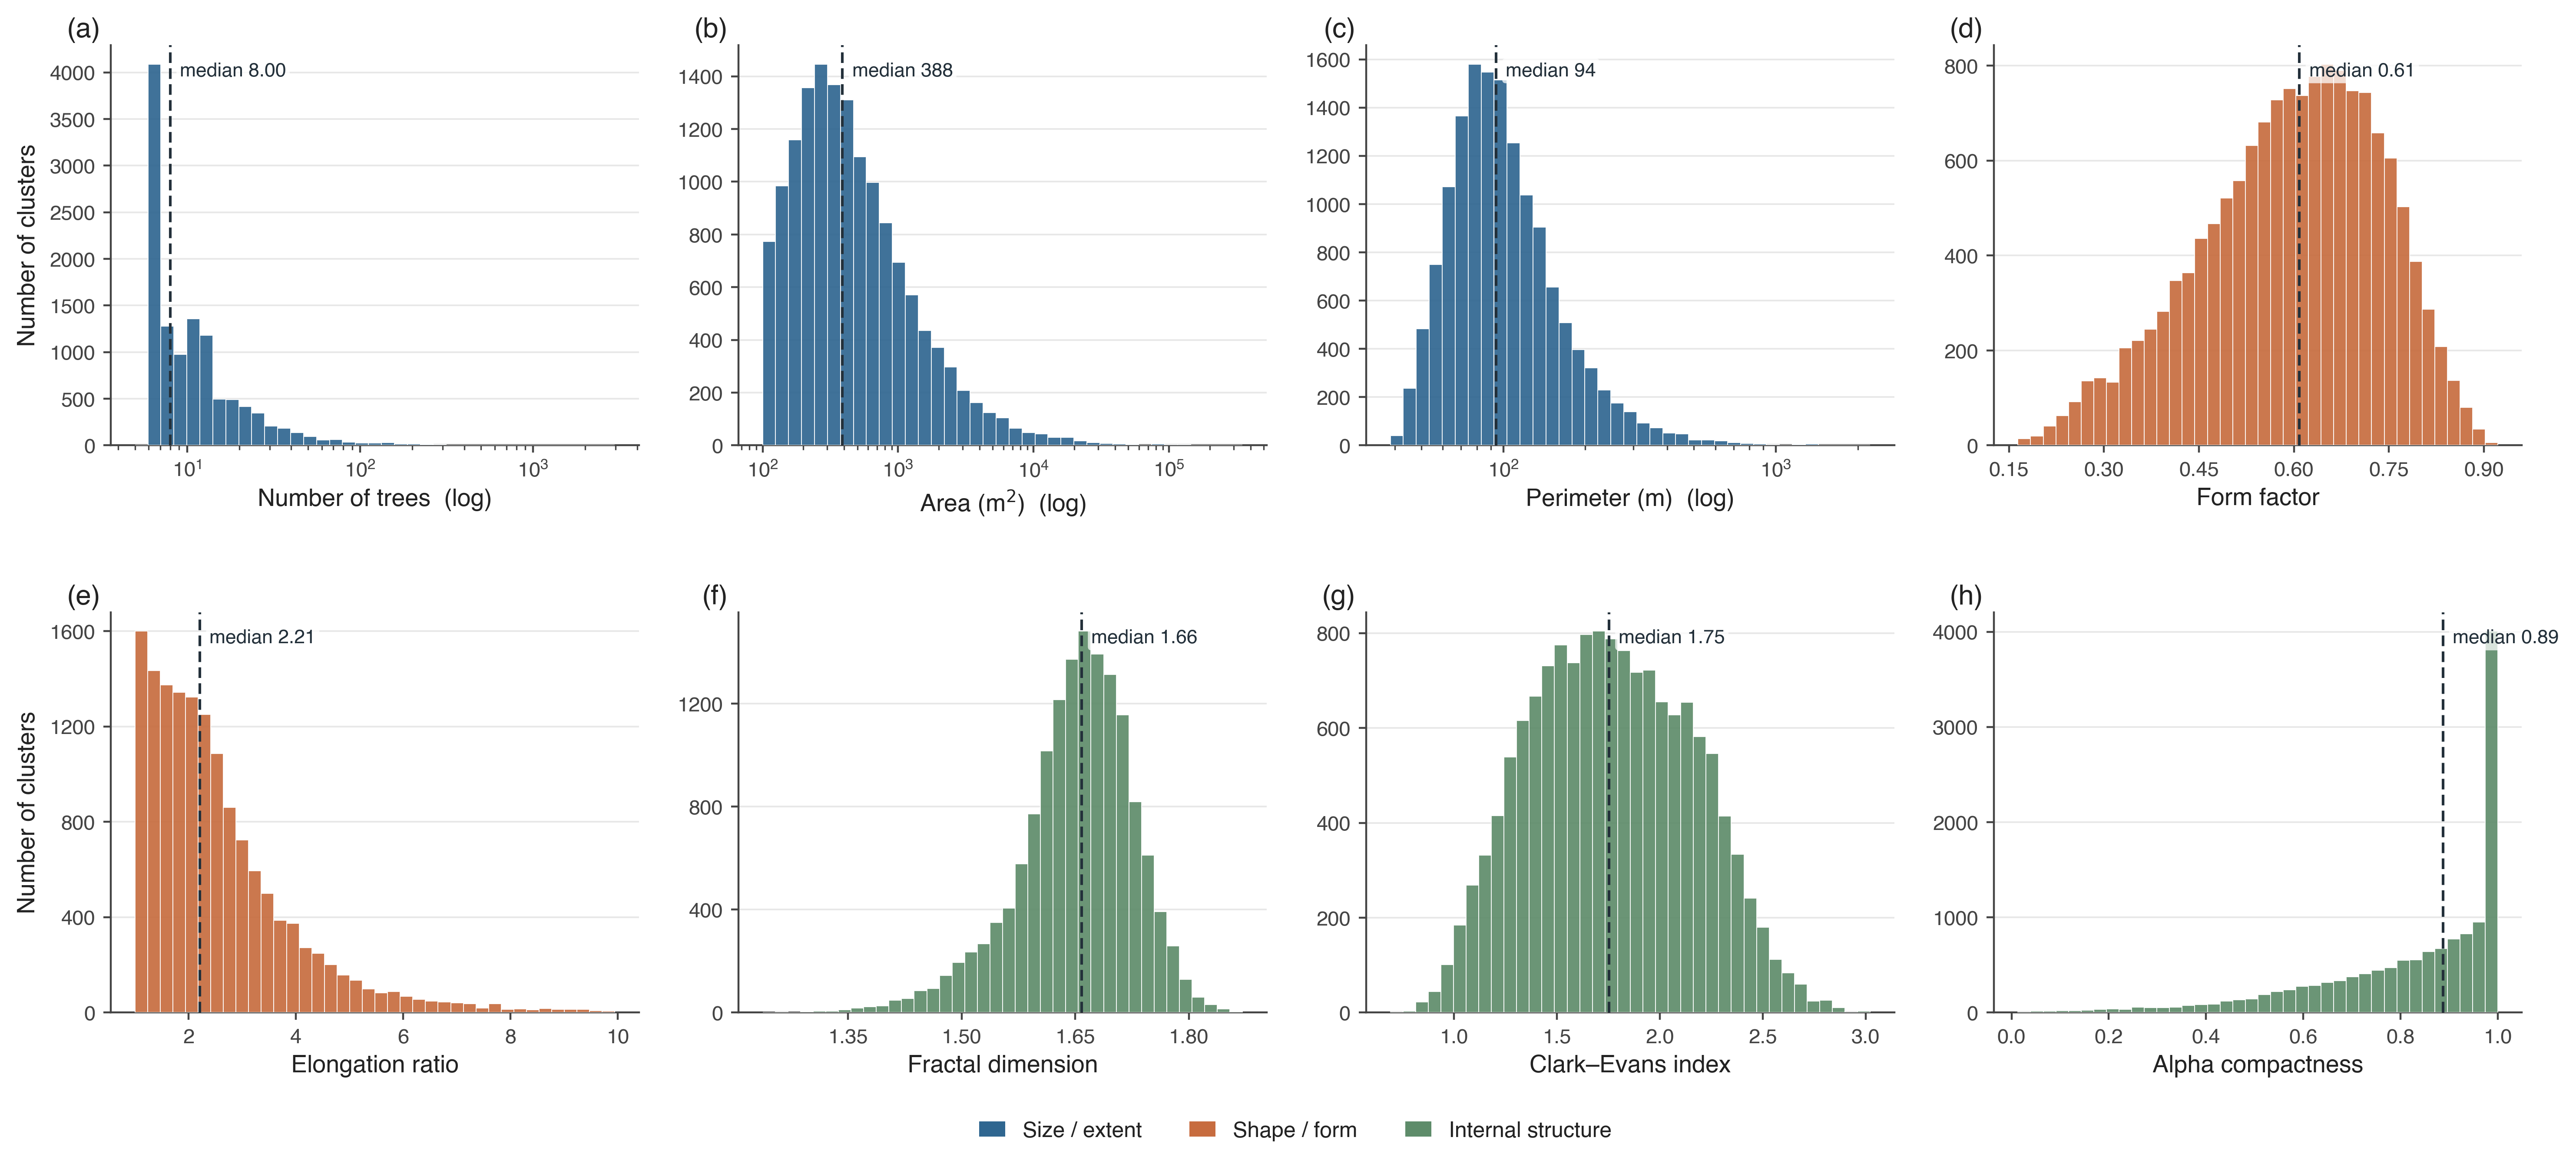
\includegraphics[width=\linewidth]{fig2_histograms.png}
  \caption{Distributions of key cluster metrics across all 14,582 clusters, coloured by metric
           family (blue: size/extent; orange: shape/form; green: internal structure). Panels
           (a)--(c) span two to three orders of magnitude and use a logarithmic x-axis with
           log-spaced bins; on this scale area and perimeter are approximately lognormal. The
           remaining panels use linear axes. Dashed lines mark per-metric medians.}
  \label{fig:histograms}
\end{figure}

The spatial distribution of all 14,582 cluster centroids across the sampled tiles is the sampling
footprint shown earlier in Figure~\ref{fig:sampling}.

\subsection{Morphological Gradient and Candidate Partition}
\label{sec:res-typology}

\mypar{K-sweep and selection.}
Among $k=2,\ldots,7$, $k=2$ gave the best combined validation performance
(silhouette\,=\,0.401, CH\,=\,8767, DB\,=\,1.073).

\mypar{Significance against a covariance-preserving null.}
The observed silhouette (0.401) exceeded the mean (0.321) and 95th percentile (0.324) of a
999-replicate null drawn from a single multivariate Gaussian matched to the observed feature
covariance, yielding $p = 0.001$ (Figure~\ref{fig:permtest}). Because this null preserves all
inter-feature correlation, the result indicates that the data are more structured than one
elongated correlated cloud, a substantially stronger statement than rejecting the
column-shuffled null, which any correlated dataset trivially beats.

\mypar{Continuum, not dichotomy.}
Gaussian-mixture BIC decreases monotonically beyond $k=2$ (BIC: $1.163\times10^5$, $1.100\times10^5$,
$1.095\times10^5$, $1.085\times10^5$, $1.074\times10^5$, $1.073\times10^5$ for $k=1,\ldots,6$),
so no two-component model is privileged; and the first principal component (60\% of variance) is
unimodal (Sarle bimodality coefficient 0.486, below the 0.555 uniform threshold). Only 2.3\% of
clusters lie within 5\% of the $k=2$ decision boundary, but this assignment cleanliness is
expected when partitioning an elongated unimodal cloud and does not imply two natural modes.
We therefore interpret the $k=2$ partition as two endpoints of a continuous
compactness--elongation gradient.

\mypar{The gradient is within-band, not a latitudinal mixture.}
Because the sample spans 60--68\textdegree{}N, across which disturbance regimes differ (beetle is
host- and temperature-limited toward the south; snow-load and wind rise in the centre; spruce
thins toward Lapland), a pooled gradient could in principle be an artefact of mixing
latitudinally-distinct regimes. It is not. Computed separately within each of the 7 sampling blocks (Table~\ref{tab:blocks}), the defining
gradient axis is essentially identical everywhere: the within-block compactness--aspect-ratio
correlation is $r \in [-0.869, -0.855]$ across all blocks, from the southern coast (60.6\textdegree{}N)
to Lapland (67.6\textdegree{}N). The compactness--elongation gradient is thus a within-block
morphological phenomenon reproduced at every site, not an artefact of pooling latitudinally-distinct
disturbance regimes. We caution that this near-constant $r$ is consistent with the trade-off being a
geometric near-tautology (both axes are hull-derived) rather than an ecological law; what it
licenses is that the \emph{form} of the relationship is region-invariant, not that the
\emph{position} of clusters along it is representatively sampled.

\begin{table}[!t]
    \def\arraystretch{1.1}
    \centering
    \footnotesize
    \caption{Per-block coverage. The compactness--aspect-ratio gradient axis is invariant across all
           seven sampling blocks; Type-0 share and block size vary. Blocks are ordered by latitude.}
    \begin{adjustbox}{max width=0.9\columnwidth}
    \begin{tabular}{llccccc}
    \toprule
    \textsc{\shortstack{Block\\(approx.\ location)}} 
    & \textsc{\shortstack{$n$ clusters}} 
    & \textsc{\shortstack{Type\,0 \%}} 
    & \textsc{\shortstack{$r$(AR, comp.)}} \\
    \midrule
    SW coast (60.6\textdegree{}N)   & 1{,}243 & 23.6 & $-0.860$ \\
    South (60.7\textdegree{}N)      & 4{,}275 & 22.7 & $-0.866$ \\
    Southeast (60.7\textdegree{}N)  & 2{,}116 & 20.0 & $-0.864$ \\
    East (61.4\textdegree{}N)       & 370     & 24.6 & $-0.855$ \\
    SE inland (62.2\textdegree{}N)  & 984     & 28.4 & $-0.869$ \\
    Central-north (65.1\textdegree{}N) & 4{,}217 & 22.8 & $-0.867$ \\
    Lapland (67.6\textdegree{}N)    & 1{,}377 & 29.3 & $-0.868$ \\
    \bottomrule
    \end{tabular}
    \end{adjustbox}
    \label{tab:blocks}
\end{table}

\begin{figure}[htb]
  \centering
  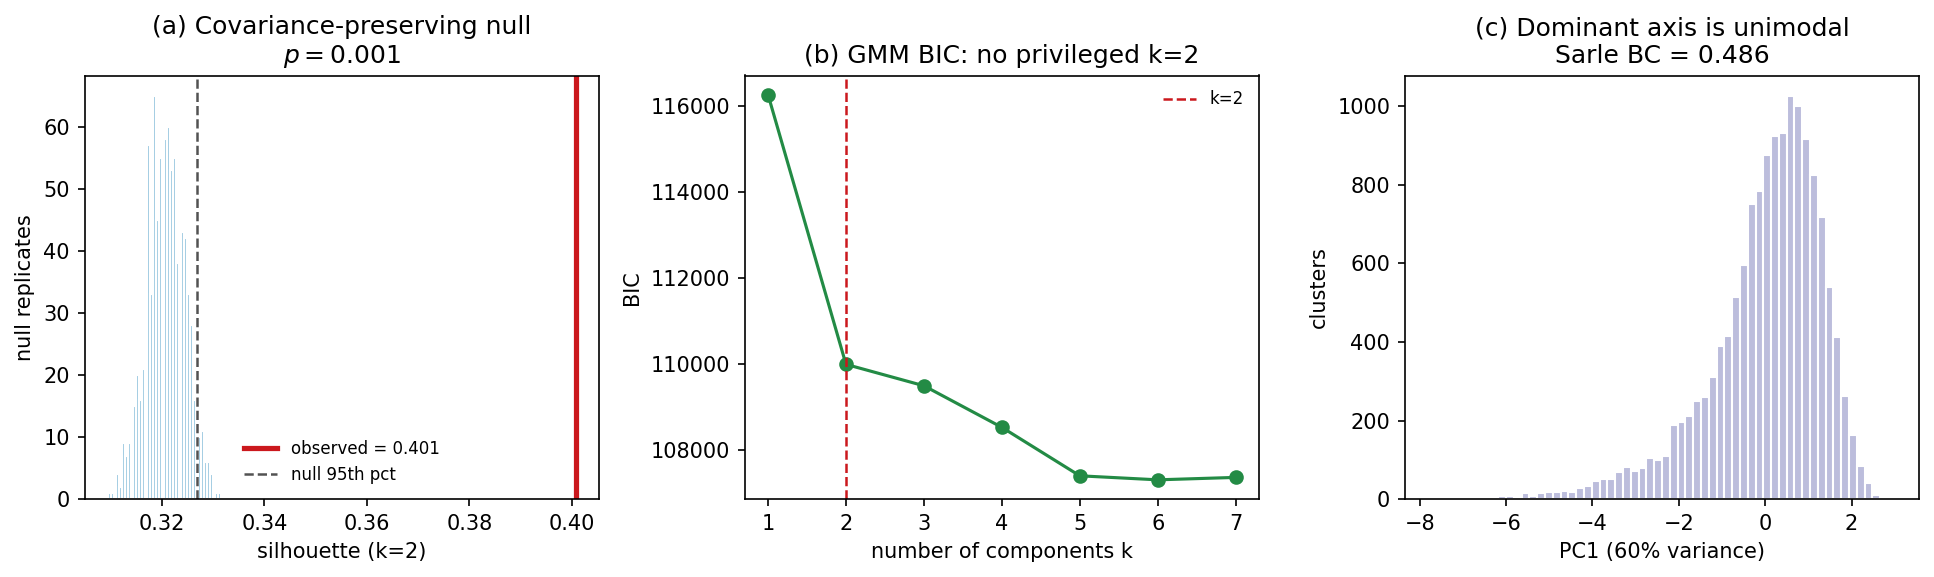
\includegraphics[width=\linewidth]{fig_silhouette_permtest.png}
  \caption{Significance and discreteness of the $k=2$ partition.
           \textbf{(a)} The observed silhouette (red line, 0.401) exceeds a 999-replicate
           \emph{covariance-preserving} null (single multivariate Gaussian matched to the feature
           covariance; mean 0.321, 95th pct 0.324), $p = 0.001$, a far stricter test than
           column-shuffling. \textbf{(b)} Gaussian-mixture BIC decreases monotonically past $k=2$,
           so no two-component model is privileged. \textbf{(c)} The first principal component
           (60\% of variance) is unimodal (Sarle coefficient 0.486). Together: real structure, but
           a continuous gradient rather than two discrete classes.}
  \label{fig:permtest}
\end{figure}

\mypar{Endpoint descriptions.}
Table~\ref{tab:types} summarises per-endpoint metric means and standard deviations.
The \textit{elongated/dispersed} endpoint (\textit{Type\,0}; 3,422 clusters, 23.5\%) is
characterised by high aspect ratio (4.291$\pm$1.490), low compactness (0.410$\pm$0.093),
and elevated Clark--Evans index (2.044$\pm$0.360). The \textit{compact/aggregated} endpoint
(\textit{Type\,1}; 11,160 clusters, 76.5\%) shows rounder, denser
shapes (compactness\,=\,0.651$\pm$0.101, AR\,=\,2.014$\pm$0.714) with higher fractal
dimension (1.679$\pm$0.051) and larger mean area (1,269\,m$^2$ vs.\ 382\,m$^2$). We use
\textit{Type\,0}/\textit{Type\,1} purely as labels for the two ends of the gradient and attach
no disturbance-agent meaning to them here.

\begin{table}[!t]
    \def\arraystretch{1.1}
    \centering
    \footnotesize
    \caption{Per-type means $\pm$ SD for all morphological features.
           Clustering was performed on fractal\_dim, clark\_evans, and aspect\_ratio only;
           the remaining features are descriptive.}
    \begin{adjustbox}{max width=0.9\columnwidth}
    \begin{tabular}{lcc}
    \toprule
    \textsc{\shortstack{Feature}}
    & \textsc{\shortstack{Type 0\\(elongated/dispersed)\\(\textnormal{$n=3,422$})}}
    & \textsc{\shortstack{Type 1\\(compact/aggregated)\\(\textnormal{$n=11,160$})}} \\
    \midrule
    Fractal dimension         & $1.555 \pm 0.069$ & $1.679 \pm 0.051$ \\
    Clark--Evans index        & $2.044 \pm 0.360$ & $1.681 \pm 0.363$ \\
    Aspect ratio              & $4.291 \pm 1.490$ & $2.014 \pm 0.714$ \\
    Compactness               & $0.410 \pm 0.093$ & $0.651 \pm 0.101$ \\
    Alpha compactness         & $0.713 \pm 0.250$ & $0.855 \pm 0.161$ \\
    Core-to-edge ratio        & $0.662 \pm 0.104$ & $0.799 \pm 0.089$ \\
    Mean NND (m)              & $8.555 \pm 2.489$ & $7.561 \pm 2.360$ \\
    Mean area (m$^2$)         & 382               & 1{,}269           \\
    Mean $n$ (trees)          & 7.7               & 15.6              \\
    \bottomrule
    \end{tabular}
    \end{adjustbox}
    \label{tab:types}
\end{table}

The spatial distribution of the two gradient endpoints within a southern display window
(one tile, 10.9\% of clusters, shown for legibility) is given in
Supplementary Fig.~S3; the inset locates this window within the national sample.


\mypar{Size-frequency distributions (E1).}
For both endpoints a lognormal cluster-size distribution is preferred over a power law
(likelihood-ratio test $p < 0.001$; \citealt{clauset2009power}). We therefore do not interpret
the nominal power-law exponents as process signatures, once the power law is rejected, its
exponent is not a meaningful mechanistic parameter. Descriptively, Type\,1 has the heavier upper
tail (Supplementary Fig.~S4), but this follows directly from its larger mean cluster area
(1,269 vs.\ 382\,m$^2$) and does not by itself imply a contagious generating process.


\mypar{Position in shape space (E5).}
Figure~\ref{fig:shapespace} plots each cluster in (compactness, aspect\_ratio) space against a
set of \emph{illustrative} morphological regions loosely informed by qualitative descriptions of
wind, beetle, and fire patches in the literature~\citep{seidl2011unraveling, jonsson2012epidemics,
gardiner2013wind}. We stress that these regions are author-defined bounding boxes, not published
(compactness, aspect\_ratio) envelopes, the cited studies do not report cluster-level shape
coordinates by agent, and that any apparent separation is partly circular: aspect ratio is a
clustering input and compactness is geometrically coupled to it. The descriptive overlaps
(Table~\ref{tab:shapespace}) therefore restate the gradient definition rather than provide
independent ecological validation, and we report them only to locate the two endpoints in a
shape space comparable to qualitative literature accounts. Establishing genuine agent
correspondence requires overlay with an independent disturbance-agent map (see Discussion).

\begin{table}[!t]
    \def\arraystretch{1.1}
    \centering
    \footnotesize
      \caption{Position of each endpoint relative to illustrative, author-defined shape regions
           (E5). These regions are not published reference envelopes and the overlaps are
           partly circular (see text); they are descriptive, not validating.}
    \begin{adjustbox}{max width=0.9\columnwidth}
    \begin{tabular}{lcc}
    \toprule
    \textsc{\shortstack{Illustrative region}} 
    & \textsc{\shortstack{Type\,0}}
    & \textsc{\shortstack{Type\,1}} \\
    \midrule
    ``Elongated'' (wind-like)    & 57.0\% & 1.2\%  \\
    ``Intermediate'' (beetle-like) & 75.0\% & 66.4\% \\
    ``Compact'' (fire-like)      & 32.3\% & 94.7\% \\
    \bottomrule
    \end{tabular}
    \end{adjustbox}
    \label{tab:shapespace}
\end{table}

\begin{figure}[htb]
  \centering
  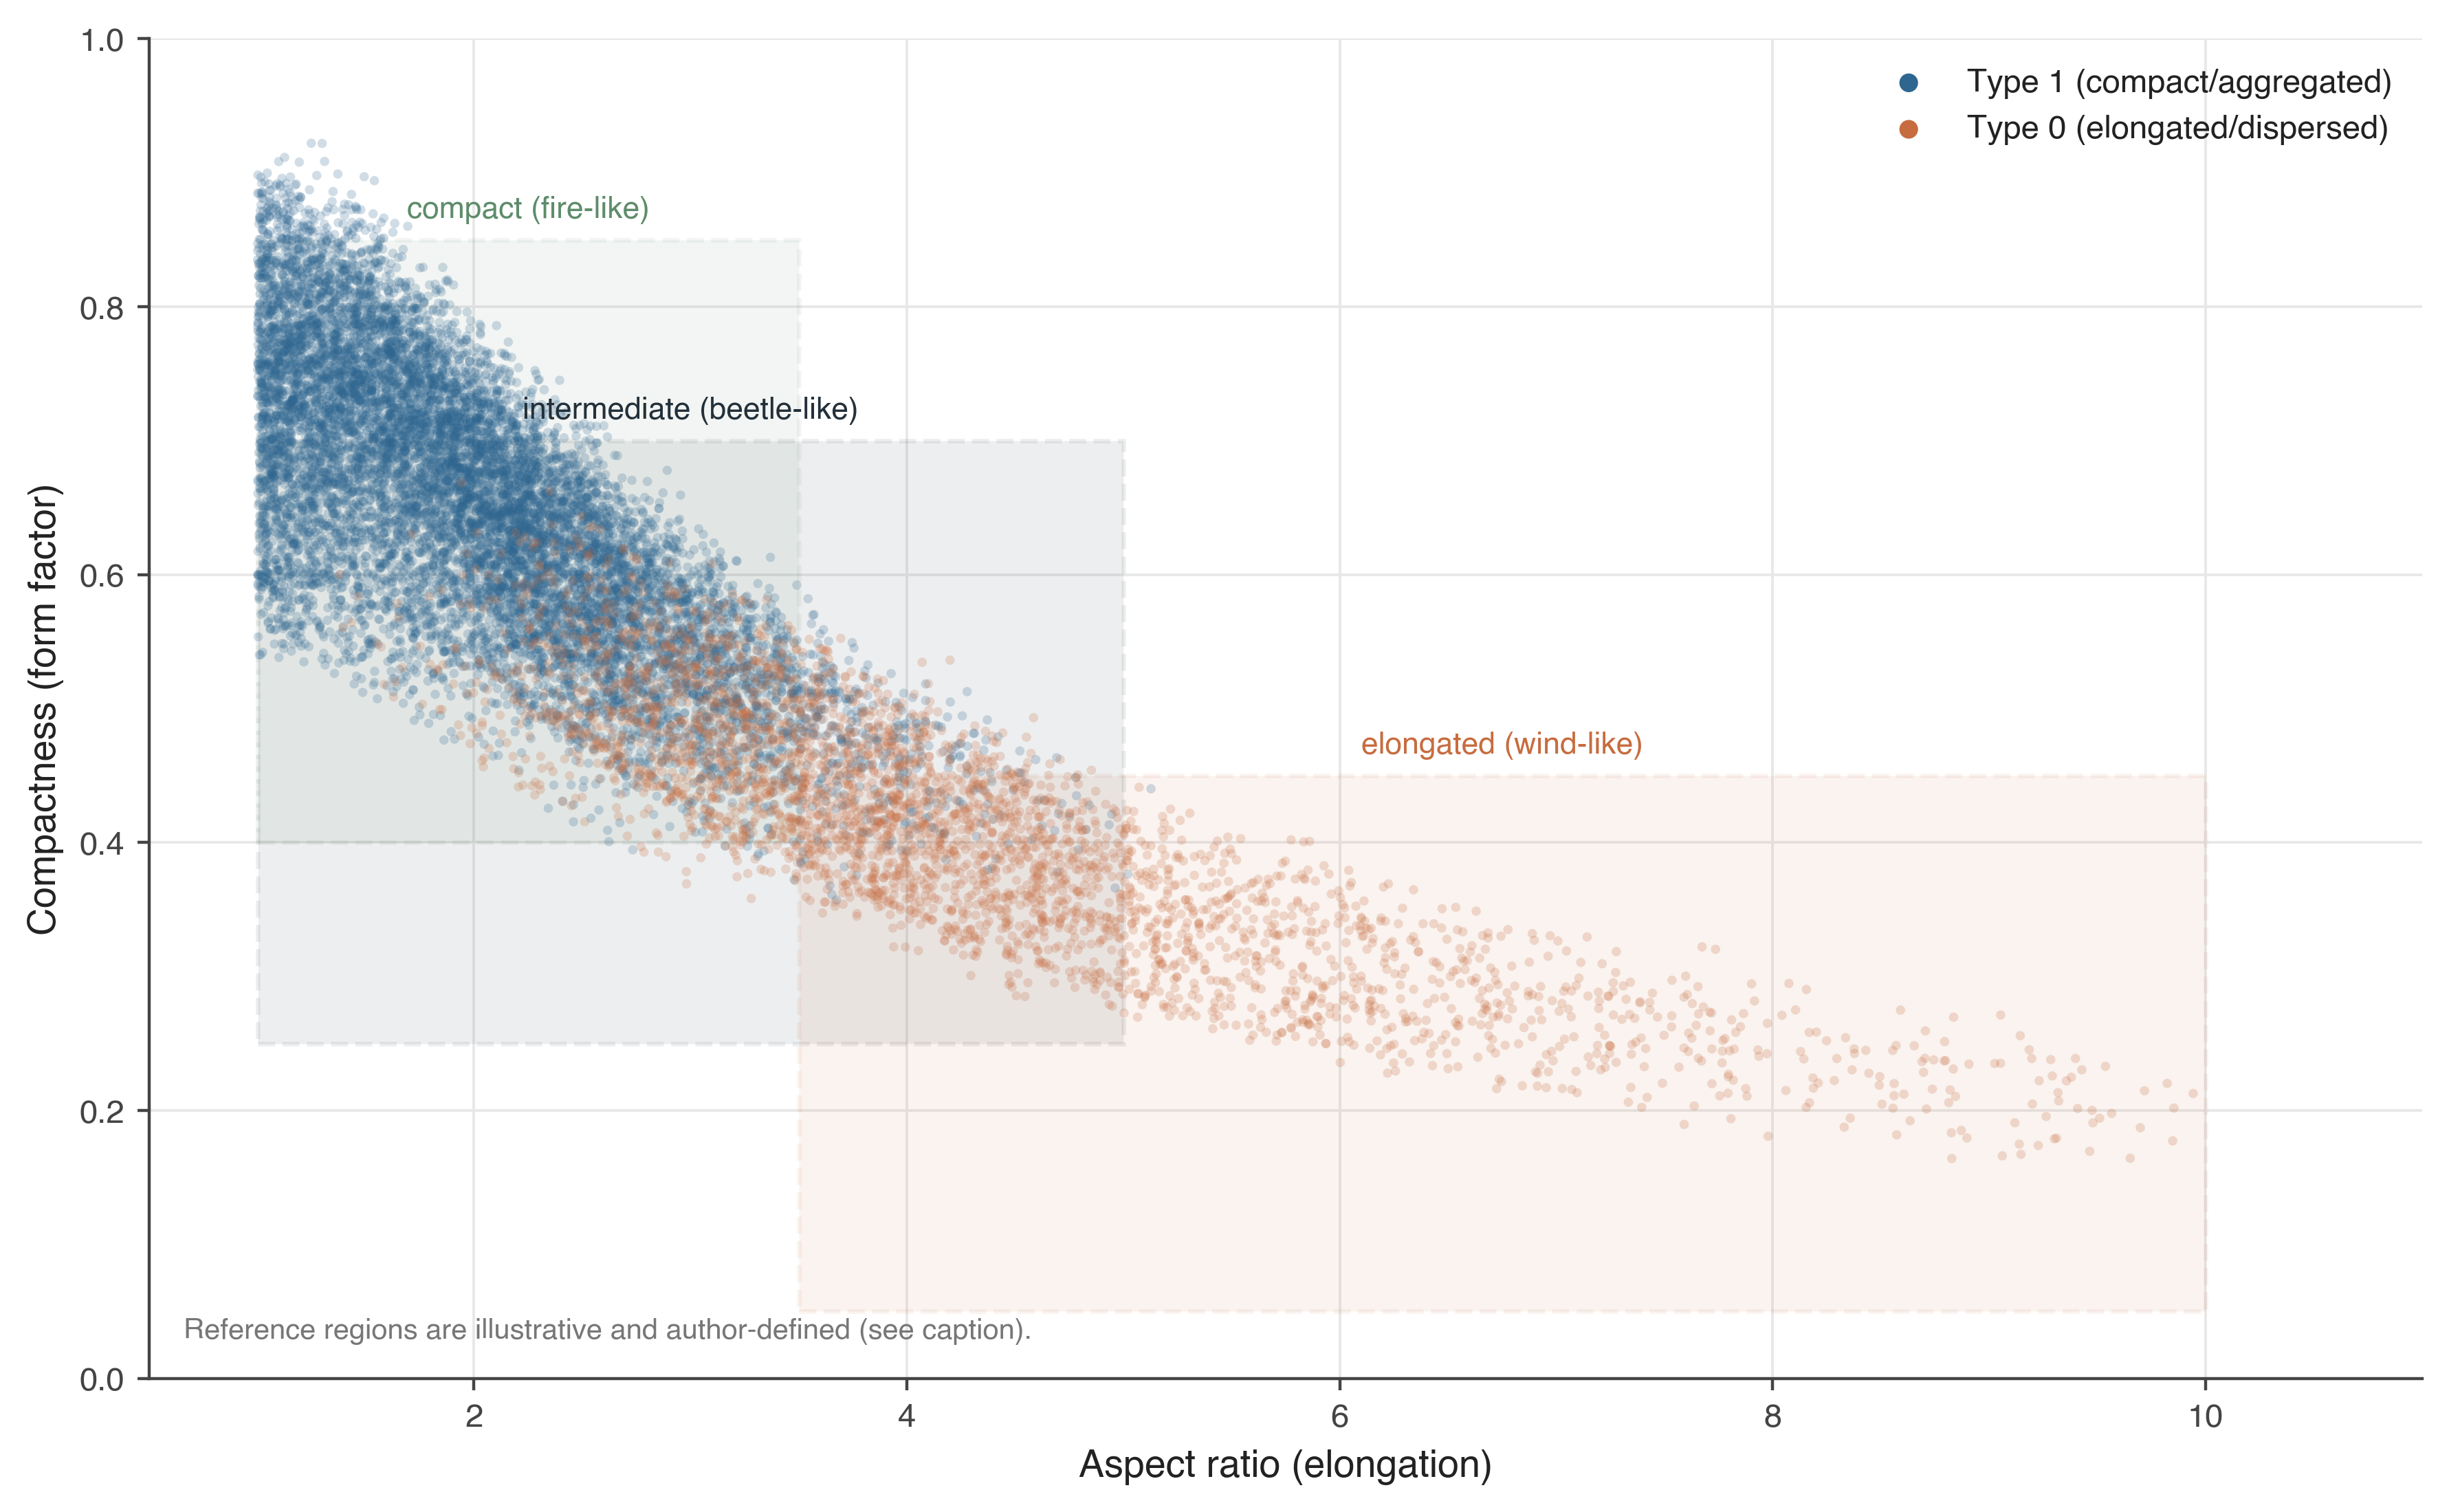
\includegraphics[width=\linewidth]{fig_shape_space.png}
  \caption{Shape-space scatter (compactness vs.\ aspect ratio) per endpoint, with
           \emph{illustrative, author-defined} shape regions overlaid. The separation is
           partly circular because aspect ratio defines the gradient and compactness is coupled
           to it; the regions are not published per-agent envelopes.}
  \label{fig:shapespace}
\end{figure}

\subsection{Orientation Analysis}
\label{sec:res-orientation}

Rayleigh tests on doubled orientation angles show no meaningful preferred direction in
either type (Figure~\ref{fig:orientation}). For Type\,0: $r = 0.009$,
mean direction\,=\,156.4°, $p = 0.747$. For Type\,1: $r = 0.040$,
mean direction\,=\,147.0°, $p = 2.0 \times 10^{-8}$. Although the Type\,1 result is
statistically significant given the large sample ($n = 11{,}160$), the mean resultant
length $r \approx 0.04$ is ecologically trivial: orientations are effectively
uniformly distributed in both types. The null orientation finding for Type\,0 is
discussed in Section~\ref{sec:disc-orientation}.

\begin{figure}[htb]
  \centering
  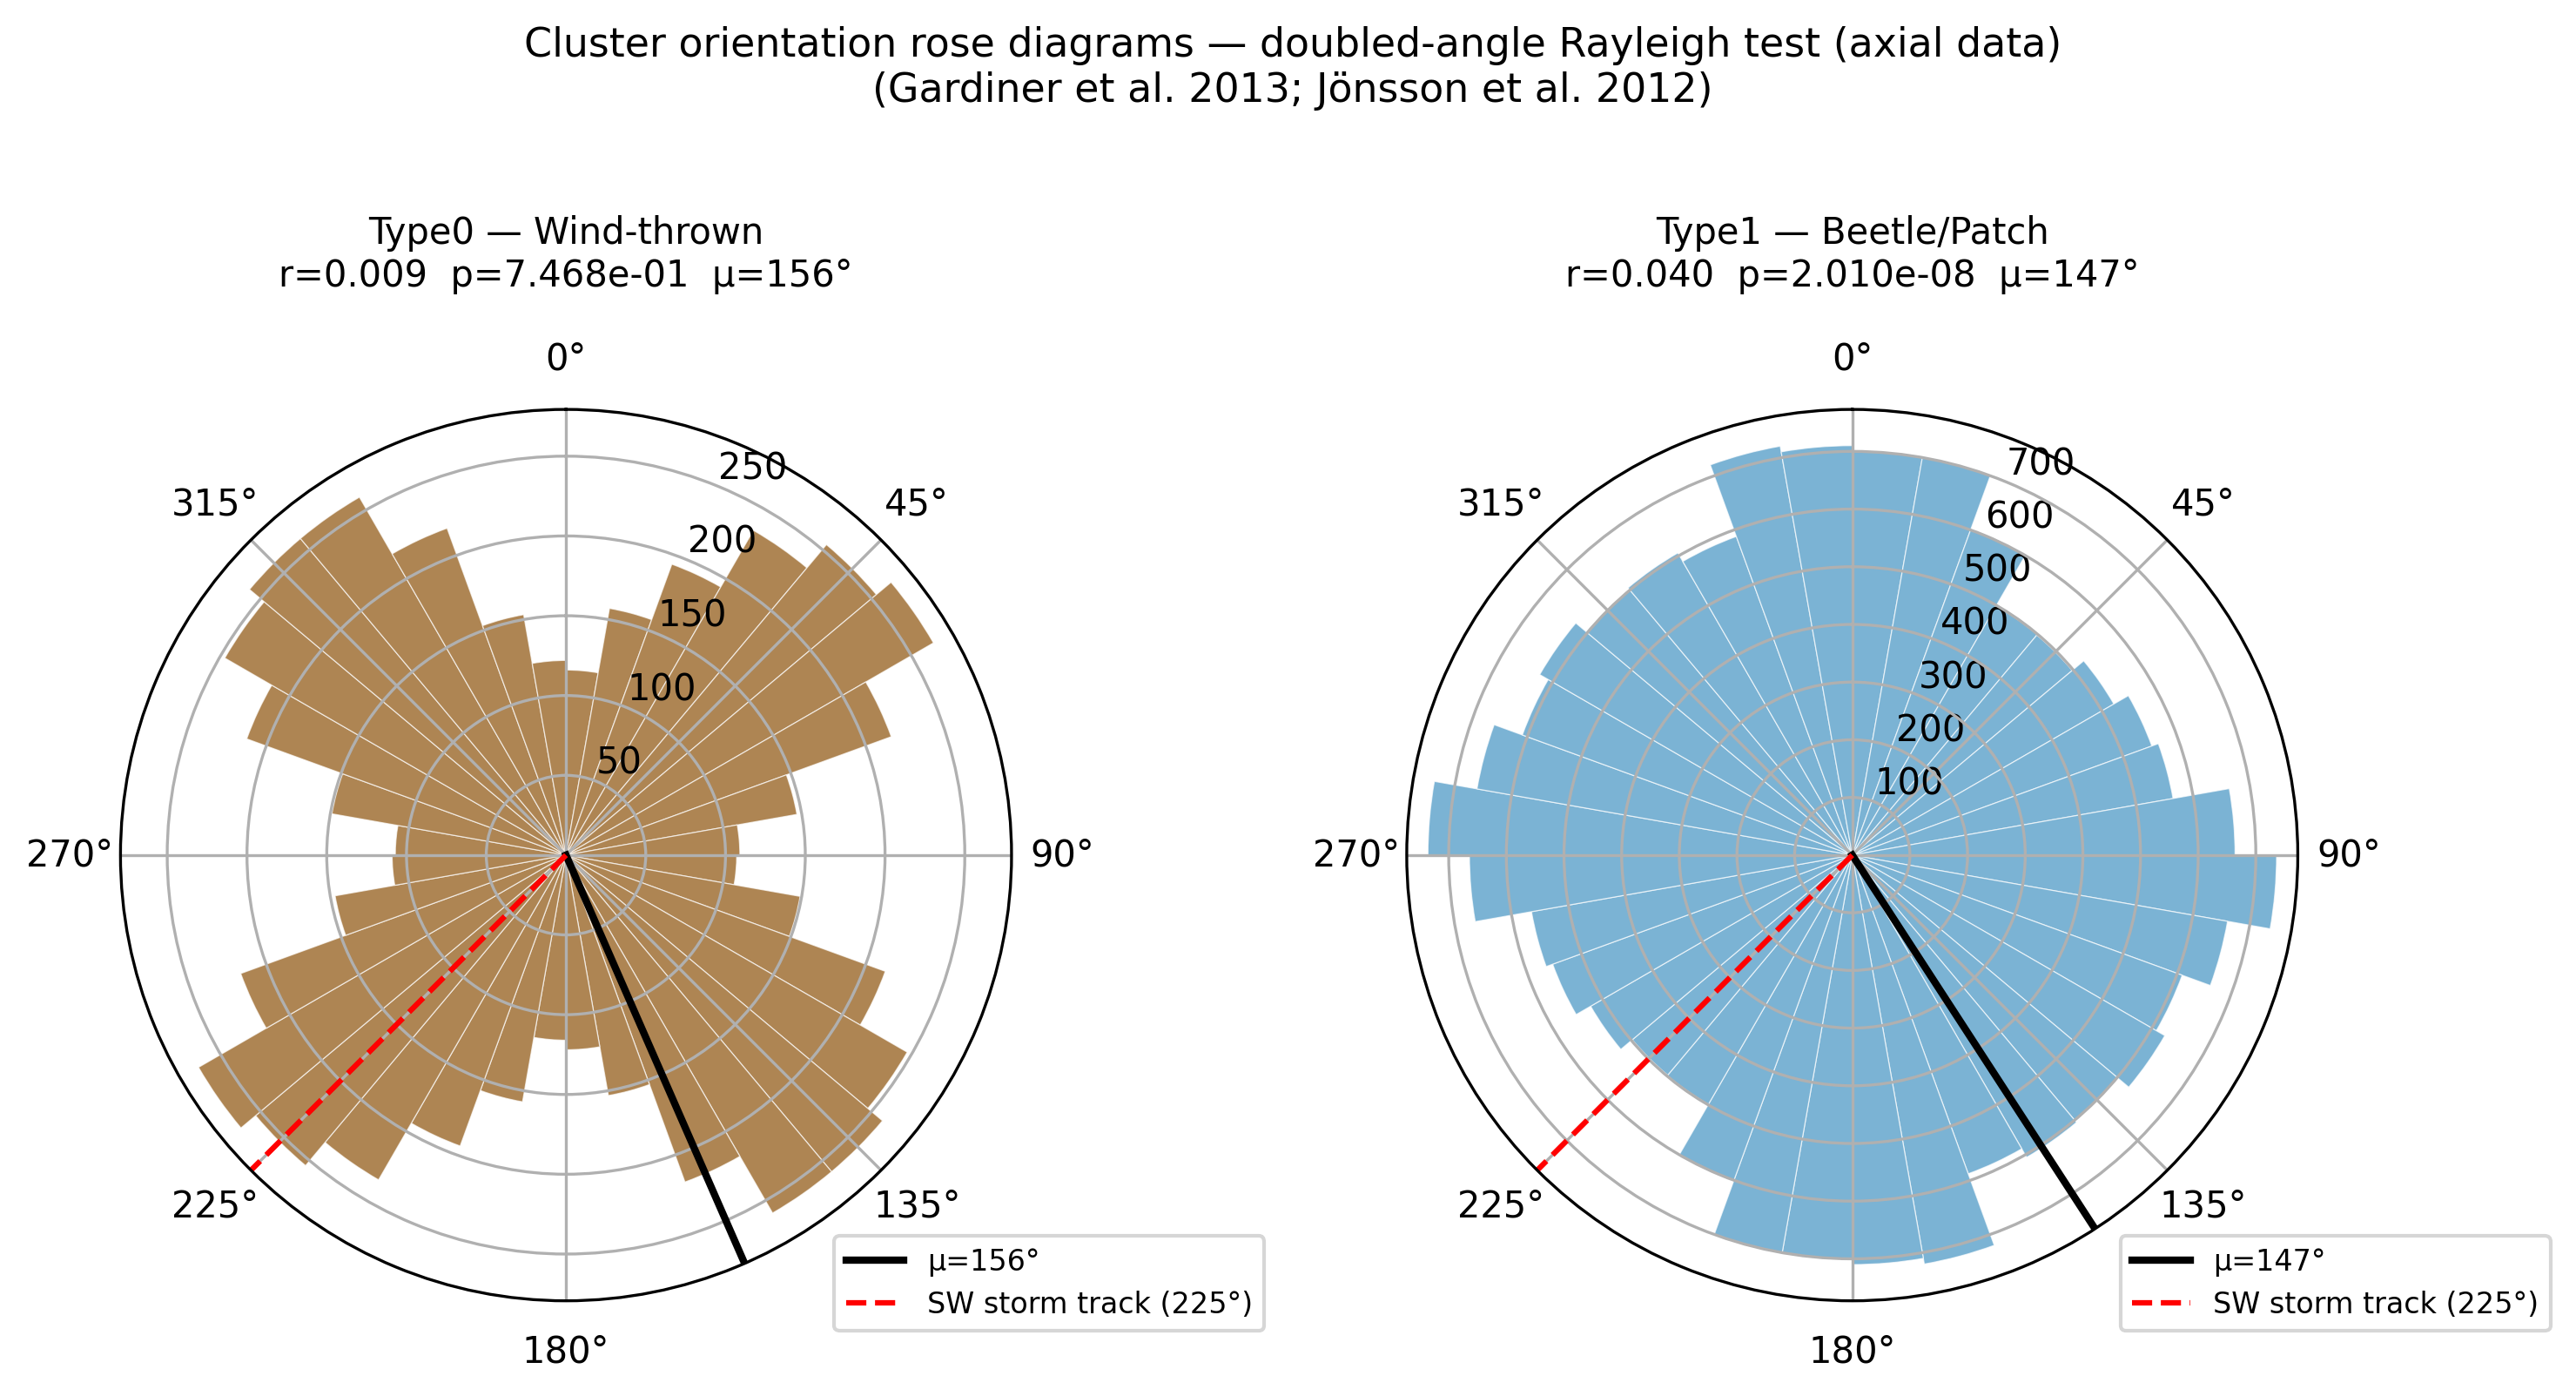
\includegraphics[width=\linewidth]{fig_orientation_rose.png}
  \caption{Polar rose plots of cluster orientation per type (axial data, 10° bins).
           Neither type shows a meaningful preferred direction ($r < 0.05$ in both cases).}
  \label{fig:orientation}
\end{figure}

\subsection{Spatial Autocorrelation}
\label{sec:res-morans}

Figure~\ref{fig:morans} presents the multi-scale Moran's $I$ heatmap (E6) for four
metrics at five distance thresholds. The autocorrelation that is present is weak in magnitude
($I \leq 0.11$ throughout). We are deliberately conservative about its significance, its
robustness, and its spatial support, for three reasons. First, under the analytical $p$-value only
Clark--Evans clears the Bonferroni threshold, and only at the 500\,m--5\,km scales; the
fractal-dimension, aspect-ratio, and compactness autocorrelations are not Bonferroni-significant.
Second, the detection-robustness gate shows that the \emph{sign} of $I$ survives a 15\%
false-negative detection perturbation for Clark--Evans, aspect ratio, and compactness ($\geq 96\%$
of realizations) but \emph{not} for fractal dimension (sign preserved in only 60--72\%), whose
near-zero autocorrelation is indistinguishable from noise once detection error is propagated.
Third, and importantly given the banded sample, the short-distance thresholds rest on very thin
support: at 200\,m, 80\% of the subsample clusters are islands (no neighbour within threshold,
mean degree 0.3), falling to 52\% at 500\,m and 0.8\% at 5\,km (mean degree 29). The nominal
``strongest at 200\,m'' cells are therefore computed on $\sim$20\% of points, whereas the
km-scale cells are well supported; this is the opposite of the usual concern that the largest
threshold is the sparsest. The defensible statement is therefore narrow: within-cluster dispersion
(Clark--Evans) shows weak but robust positive spatial autocorrelation at the well-supported
1--5\,km scale, while the shape metrics show at most marginal, detection-sensitive structure.
Because the sample is in discrete latitudinal bands separated by large gaps, all distance-band
weights connect only within-band neighbours: the reported autocorrelation is a \emph{within-band}
quantity, and between-band (latitudinal) structure is unsampled rather than absent. LISA maps (Supplementary Fig.~S5) illustrate the spatial
structure of fractal-dimension autocorrelation within the southern display window; labels are
computed on the full survey dataset to preserve correct neighbourhood weights, and given the
weak global signal for this metric they are best read qualitatively.

\begin{figure}[htb]
  \centering
  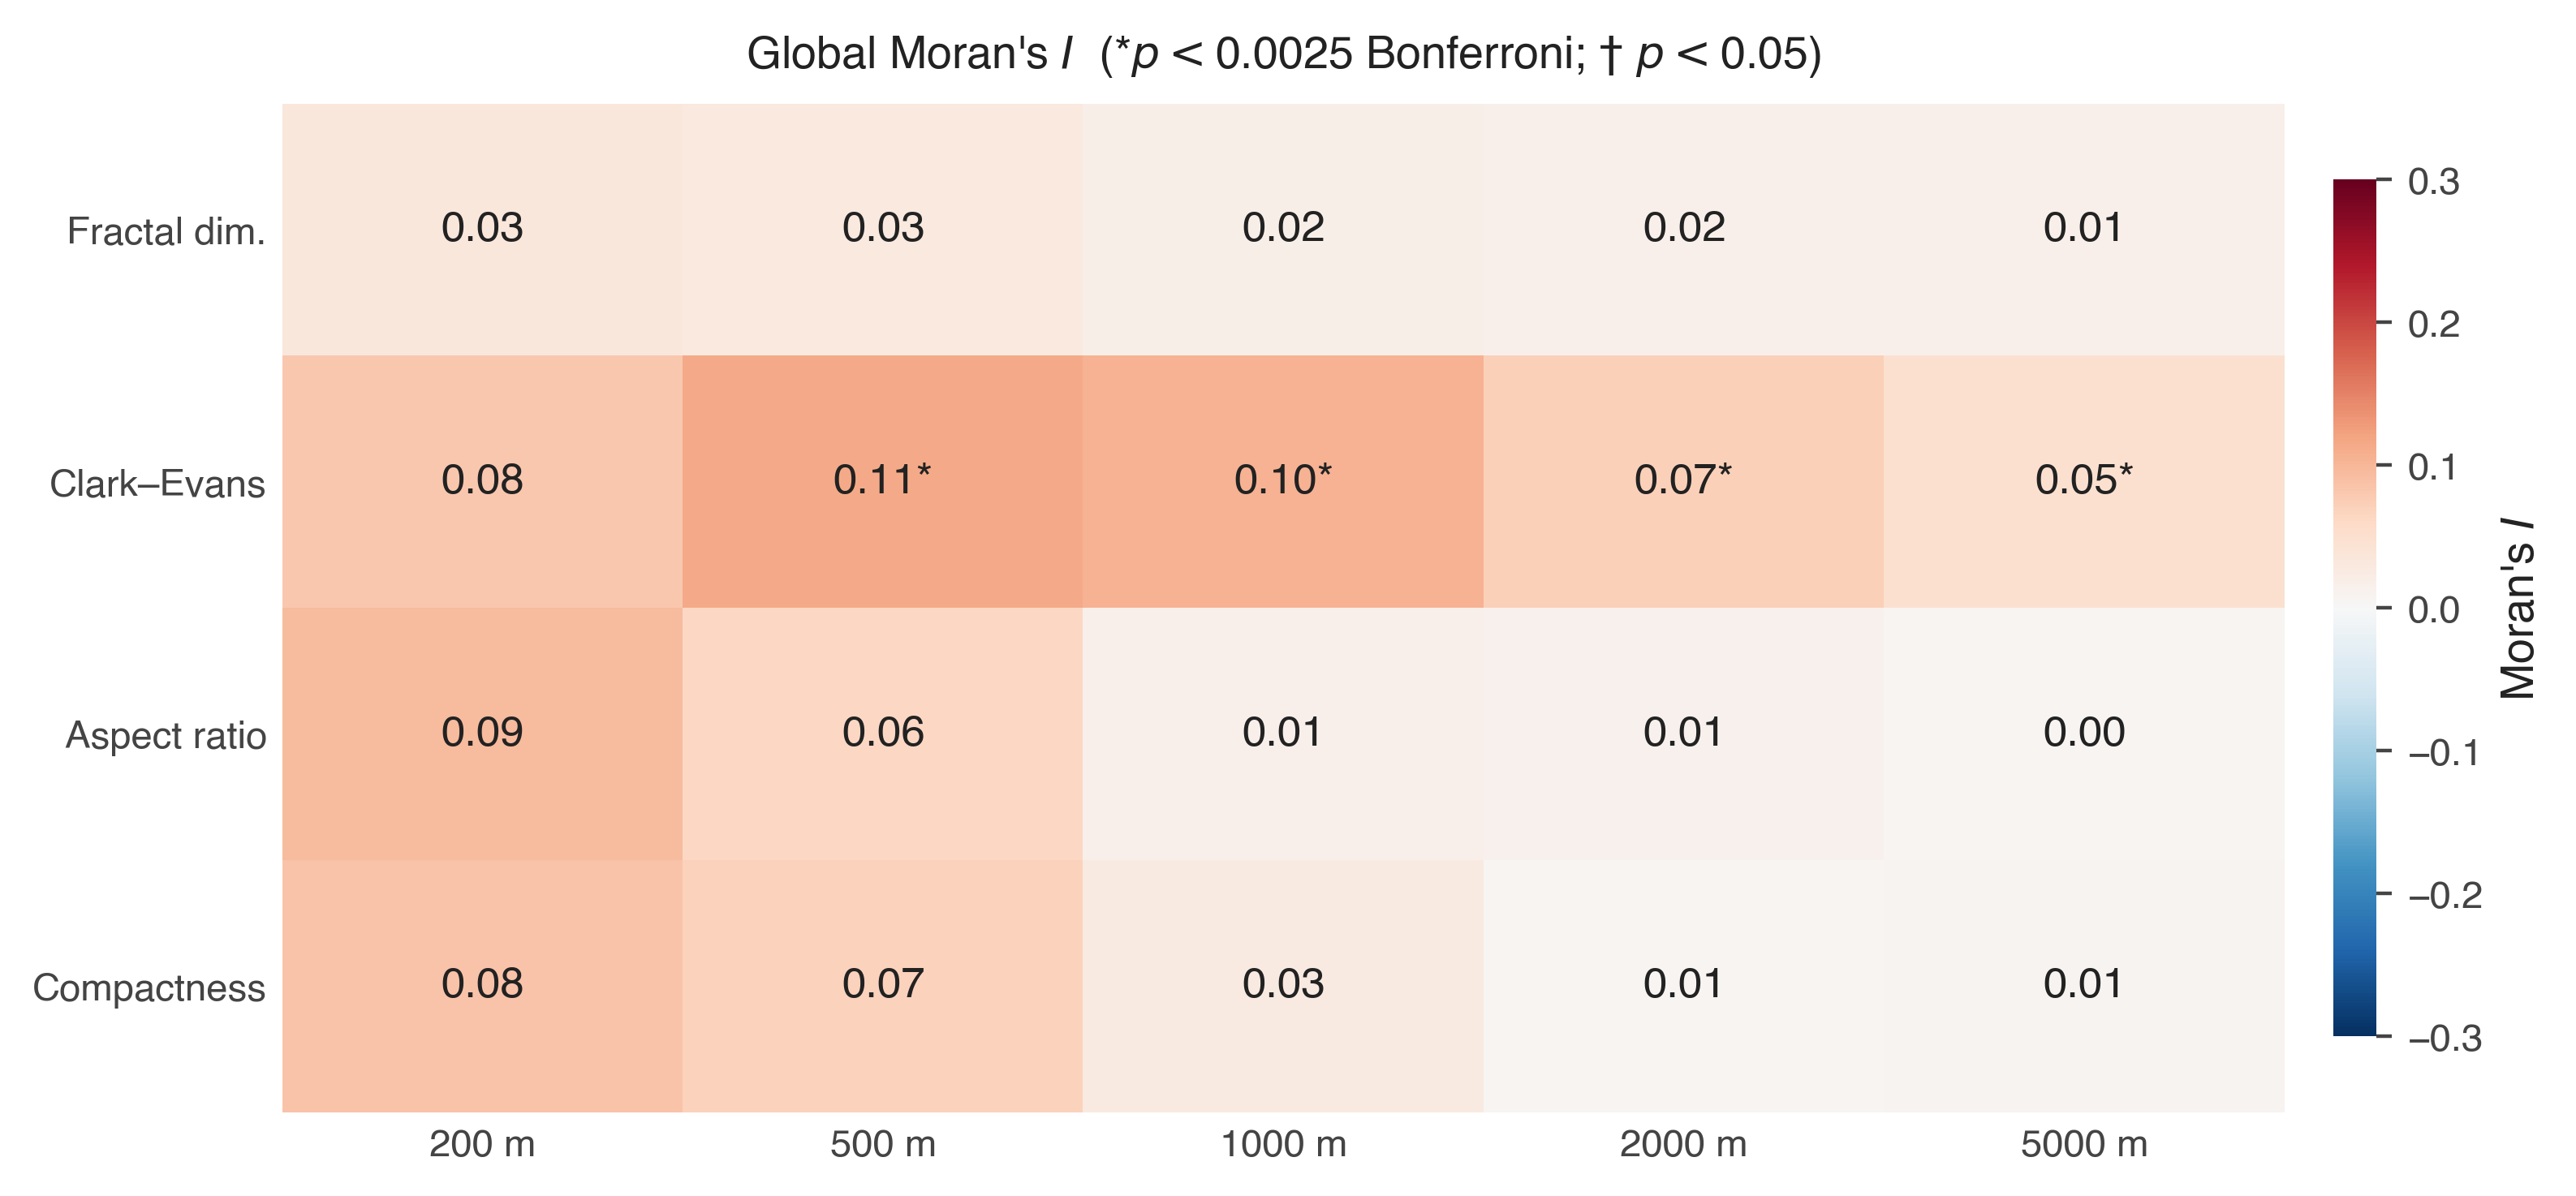
\includegraphics[width=\linewidth]{fig_moran_heatmap.png}
  \caption{Moran's $I$ heatmap (E6): four metrics (rows) $\times$ five distance
           thresholds (columns), analytical $p$. Cells marked $*$ clear the Bonferroni
           threshold $\alpha^* = 0.0025$, $\dagger$ are nominally significant ($p<0.05$).
           Autocorrelation is weak throughout ($I \leq 0.11$); only Clark--Evans is
           Bonferroni-significant (1--5\,km), and a 15\% false-negative detection perturbation
           leaves the sign of $I$ stable for all metrics except fractal dimension. The 200\,m
           column rests on $\sim$20\% of points (80\% islands); km-scale columns are well
           supported. Weights connect within-band neighbours only.}
  \label{fig:morans}
\end{figure}


\subsection{Landscape Connectivity}
\label{sec:res-connectivity}

At the 200\,m threshold, the proximity graph over all clusters contains 13,351 edges; the largest
connected component spans only 175 of 14,582 clusters and roughly a third of clusters are
isolated singletons, so the graph is sparse. Supplementary Fig.~S6 shows connectivity
reach and bridge clusters within the southern display window (statistics from the full graph).
Pooled across all clusters, Type\,1 appears more connected than Type\,0 (median reach\,=\,3 vs.\ 2;
mean reach 11.03 vs.\ 8.98; Mann--Whitney $p = 1.7\times10^{-10}$), but this is a pseudoreplication
artefact: the rank-biserial effect size is only $r = 0.07$, and the test treats 14,582
block-nested clusters as independent. Tested honestly at the level of the 7 sampling blocks, the
difference does not survive: only 2 of 7 blocks show Type\,1\,$>$\,Type\,0 median reach (sign test
$p = 0.45$). The pooled ``significance'' was entirely a large-$n$ effect, and what difference exists
is a direct consequence of Type\,1's larger area and denser packing (larger, denser clusters are
mechanically more likely to fall within 200\,m of a neighbour). We therefore treat reach as a density correlate,
not an independent line of evidence. Because the graph is untimed and unweighted, we do not
interpret high-betweenness clusters as outbreak corridors or sentinels; they are geometric
articulation points whose ecological relevance is untested. We also note that, because the sample
is in discrete blocks separated by far more than 200\,m, no connected component can bridge blocks:
reach is a strictly within-block measure of local packing density and carries no between-region
connectivity meaning by construction. A meaningful connectivity analysis
would require a graph whose length scale is matched to a dispersal process, for a bark-beetle
hypothesis, a host-conditioned, dispersal-weighted graph at the $\sim$250\,m--1\,km scale of
\textit{Ips typographus} flight; for wind, storm-front co-occurrence at the tens-of-kilometre
scale of a storm footprint, and these are mutually incompatible graphs, which is itself why a
single undirected 200\,m graph cannot adjudicate either process.


\subsection{Feature-Space Coherence Check}
\label{sec:res-validation}

The held-out Random Forest classifier achieved AUC\,=\,0.976\,$\pm$\,0.002
(range 0.973--0.978 across 5 spatial folds; Supplementary Fig.~S7); re-running the cross-validation
with the 7 sampling blocks as the grouping variable (leave-one-block-out), which matches the true
spatial-dependence structure, gives an essentially identical AUC\,=\,0.975\,$\pm$\,0.003. We caution
against reading this as independent validation. The ``held-out'' features are geometrically coupled to the
K-means inputs: compactness, for example, correlates with aspect ratio at $r = -0.865$ and alone
attains a univariate AUC of about 0.96, so a high AUC is largely a restatement of the K-means
boundary through correlated geometry rather than corroboration from new information. We report it
only as an internal coherence check; on an imbalanced 76.5/23.5 partition, ROC-AUC should in
future be complemented by precision--recall AUC and per-class recall.

SHAP mean absolute values ranked features as follows:
compactness (0.226) $>$ core\_to\_edge\_ratio (0.068) $>$ nnd\_mean (0.037)
$>$ orientation (0.034) $>$ alpha\_compactness (0.019) $>$ nnd\_std (0.010)
$>$ reach\_200m (0.005).
Compactness dominates because it is geometrically correlated with aspect ratio
(a K-means input). Crucially, reach\_200m, the only feature in this set that is
independent of cluster shape, ranks last, confirming that high AUC is primarily
driven by correlated shape dimensions rather than landscape connectivity.

This same asymmetry is what licenses reporting the gradient while withholding the discrete
typology. The detector confound (G4) predicts the \emph{discrete} type at AUC\,=\,0.727, yet a
cluster's position along the \emph{continuous} gradient (first principal component of the three
features) correlates with detection confidence at only $\rho = 0.07$. The discrete labels sit
close to the detector's decision surface; the continuous morphospace coordinate does not. The
gradient is therefore the level at which the signal is least entangled with the instrument, and
the typology is the level at which it is most entangled, hence the former is reported and the
latter withheld.

Because the sample spans 60--68\textdegree{}N, we further checked whether this detector confound is
merely a latitudinal gradient (canopy composition, solar geometry, and snow/phenology all vary with
latitude and could structure detector recall). It is not: cluster location alone (easting, northing)
predicts type at AUC\,=\,0.519, essentially chance, consistent with the near-constant Type\,0
prevalence across latitude bands (22.9\%, 22.8\%, 29.3\% from south to north), and the detector
confound is unchanged when location is partialled out (AUC 0.727\,$\to$\,0.720). The confound is thus
driven by detection covariates (confidence, density), not by geography, and the morphological
gradient is not a latitudinal climate proxy.


\subsection{Stability Gates}
\label{sec:res-sensitivity}

The four gates jointly indicate that the $k=2$ split is not a discrete typology but a
convenience cut through a continuous gradient, and that one of its endpoint labels is
unsupported.

\mypar{(G1) The partition is not scale-stable.}
Re-clustering from raw across eps $\in \{10,\ldots,40\}$\,m, the Type\,0 fraction slides
monotonically (28.6\% at 10\,m, 25.8\%, 23.5\% at 20\,m, 24.0\%, 23.4\%, 22.9\% at 40\,m) and the
Type\,0 centroid drifts continuously rather than holding position (aspect ratio 2.97\,$\to$\,4.29\,$\to$\,4.79;
compactness 0.544\,$\to$\,0.410\,$\to$\,0.372 across eps 10/20/40\,m). A genuine class would be
eps-invariant; this rescaling with the clustering radius is the signature of detection chaining, not
a fixed disturbance class. BIC favours more than two components at every eps.

\mypar{(G2) The headline prevalence is an artefact of the AR cap.}
Re-clustering from raw at eps\,=\,20\,m with no AR cap (14,644 clusters) and sweeping the cap shows
the Type\,0 fraction is conditional on where the cap falls: 33.1\% (AR\,$\leq 5$), 27.0\% ($\leq 7$),
23.5\% ($\leq 10$, the published value), 21.8\% ($\leq 15$), down to 21.3\% (uncapped). The within-Type\,0
AR distribution is pressed against the cap (maximum 9.94 at AR\,$\leq 10$) and, once released, extends
as a single smooth tail to AR\,$\approx 30$ with no second mode. Membership ARI against the AR\,$\leq 10$
partition decays monotonically as the tail is restored (1.00\,$\to$\,0.92\,$\to$\,0.89). Aspect ratio is
therefore a continuum, and the AR\,$\leq 10$ cap manufactured the clean ``23.5\%'' figure
(Figure~\ref{fig:sensitivity} summarises G1 and G2).

\mypar{(G3) No directional signal beyond hull shape.}
Within matched hull-AR bins, Type\,0 and Type\,1 have statistically indistinguishable point-scatter
linearity (Figure~\ref{fig:anisotropy}; e.g.\ AR\,$\in(2,2.5]$: 0.829 vs.\ 0.830, $p=0.86$;
AR\,$\in(3,4]$: 0.916 vs.\ 0.915, $p=0.73$; Type\,1 marginally higher in the (2.5,\,3] bin). The
overall impression that Type\,0 is ``more linear'' (Figure~\ref{fig:anisotropy}a) is entirely a
hull-AR effect; once hull elongation is controlled (Figure~\ref{fig:anisotropy}b) the elongated
endpoint carries no extra line-like (wind-swath) structure. Together with the orientation null
(Section~\ref{sec:res-orientation}), this empirically removes the basis for a ``wind-thrown''
interpretation.

\begin{figure}[htb]
  \centering
  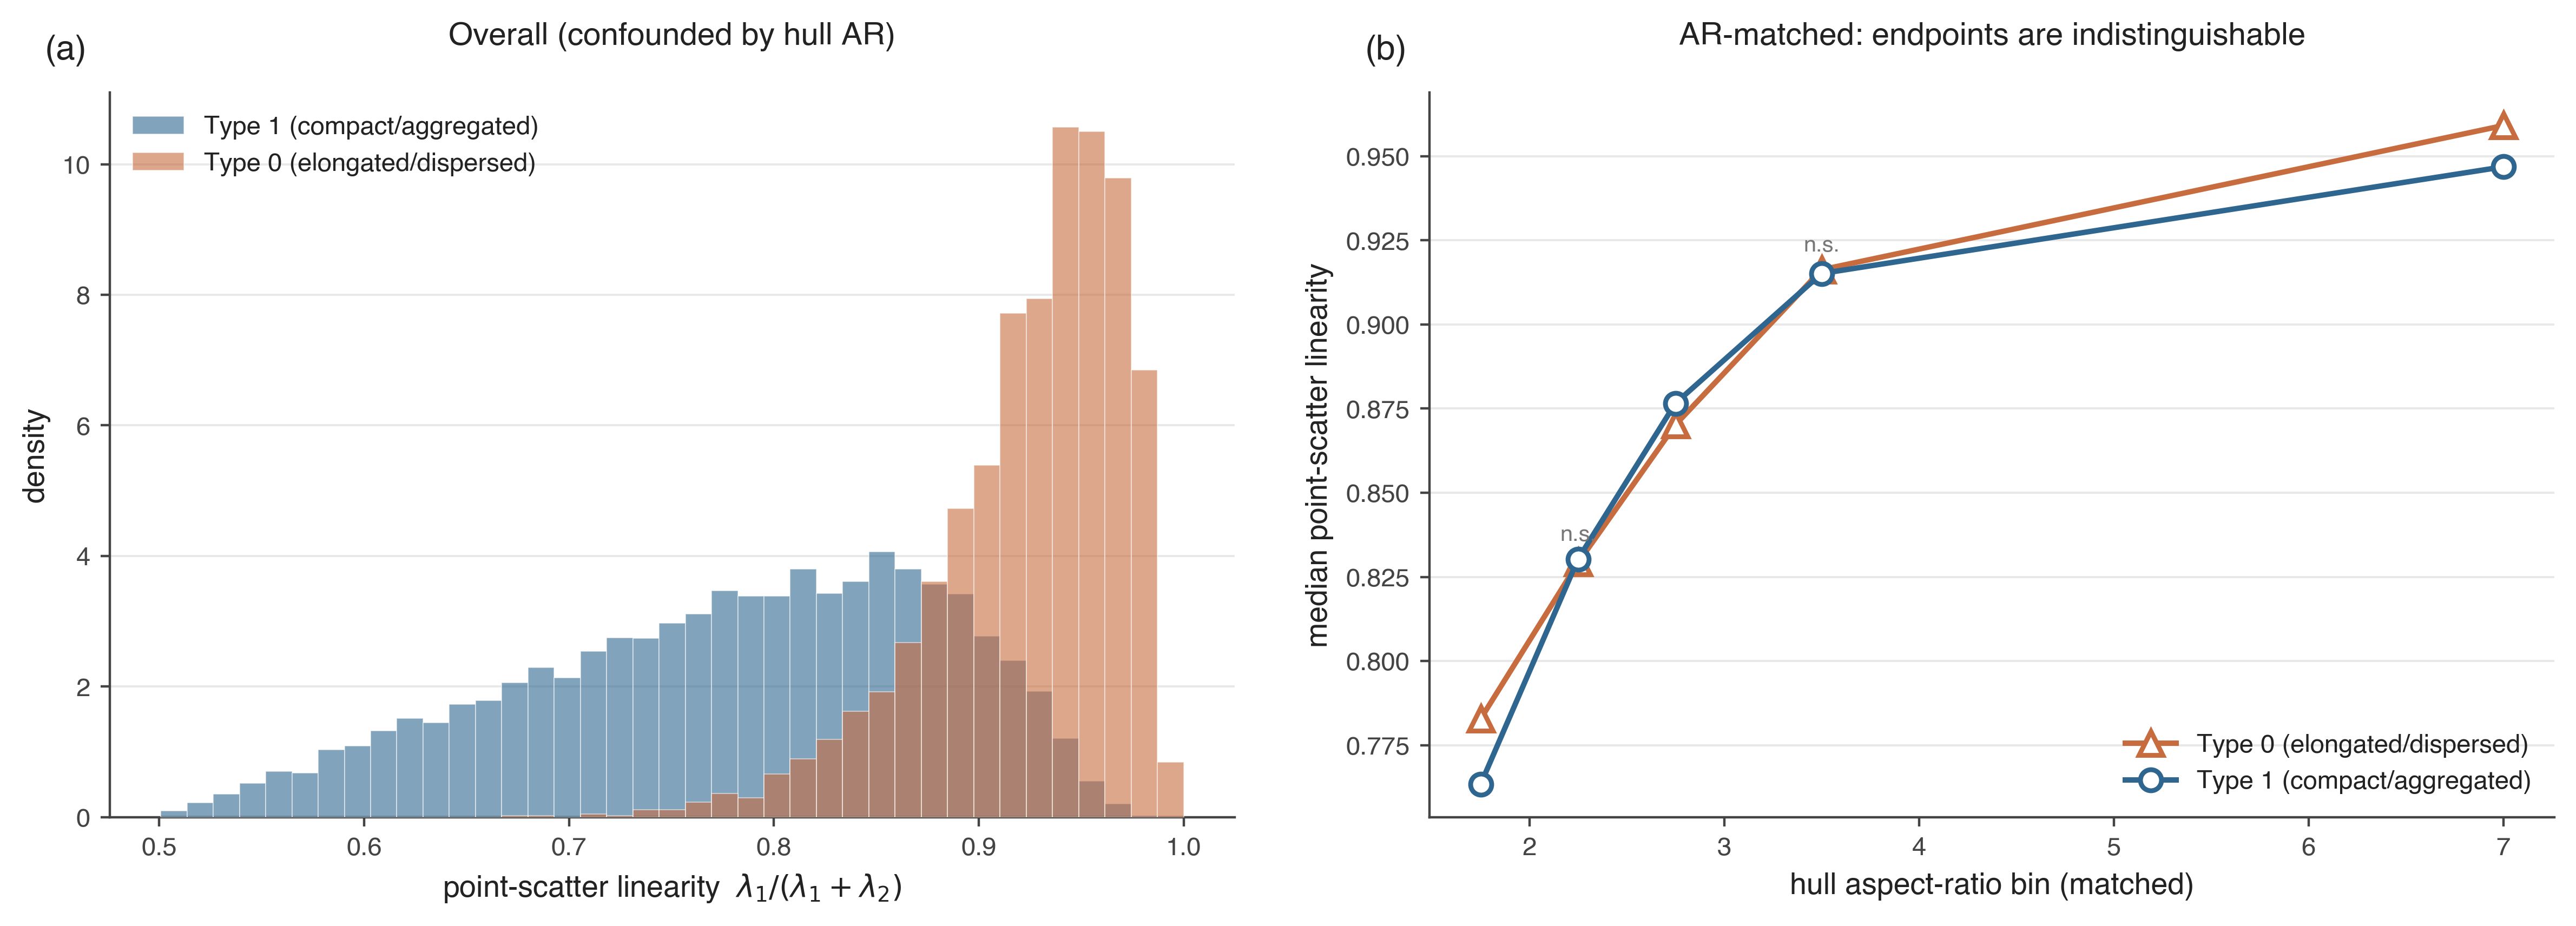
\includegraphics[width=\linewidth]{fig_anisotropy.png}
  \caption{Second-order anisotropy gate (G3). \textbf{(a)} Overall, the elongated endpoint
           appears more linear, but this is confounded by hull aspect ratio. \textbf{(b)}
           Matched on hull aspect ratio, the two endpoints' median point-scatter linearity is
           indistinguishable (n.s.\ where shown), so the elongated endpoint carries no directional
           point-process signal beyond hull shape.}
  \label{fig:anisotropy}
\end{figure}

\mypar{(G4) A measurable detector confound.}
Per-cluster detection-confidence covariates predict type at AUC\,=\,0.727 (5-fold), and dropping
10--20\% of detections per cluster flips the type of 5.9--7.5\% of clusters (ARI 0.76--0.70). The
typology is thus partly entangled with detector behaviour; cleanly separating the two requires
stratified detection precision/recall against ground truth, which the present data lack.

\begin{figure}[htb]
  \centering
  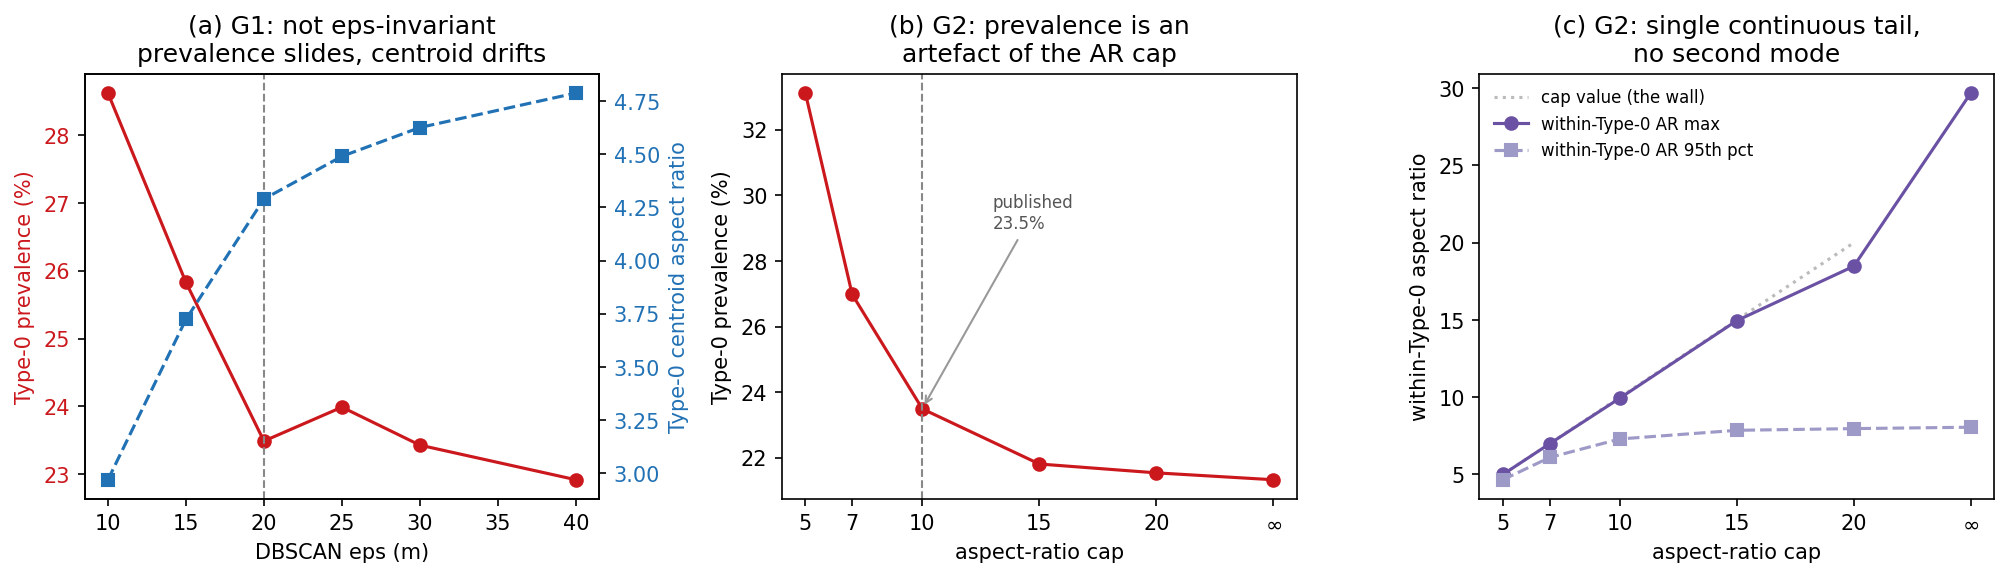
\includegraphics[width=\linewidth]{fig_dbscan_sensitivity.png}
  \caption{Stability gates. The Type\,0 fraction is not invariant to DBSCAN eps (G1) and is
           conditional on the aspect-ratio cap (G2); the elongated endpoint's AR distribution forms a
           single continuous tail once the cap is released, with no second mode.}
  \label{fig:sensitivity}
\end{figure}

\subsection{Host-Conditioned Aggregation of Mortality}
\label{sec:res-host}

This is the primary analysis. Fitting the pixel-Poisson intensity model on the forest grid, mortality
intensity increases with \emph{both} spruce and total growing-stock volume (standardised log-linear
coefficients $+0.23$ and $+0.21$ respectively; stand-edge proximity negligible, $-0.02$): canopy
mortality strongly tracks forest host availability, as expected.

Beyond this host-tracking, mortality is \emph{still} aggregated more than the host predicts at short
range. Against a spruce-only host null, the inhomogeneous $L$-function (a standard measure of how
clustered points are, here calibrated against the host surface rather than against an even scatter)
lies far above the host-conditioned envelope (the band of values expected if mortality merely
followed host) across 100\,m--1\,km (Figure~\ref{fig:hostcond}a). Crucially, the signal
survives the richer null: with intensity conditioned on spruce, total volume, and stand edge, the
observed $L_{\rm inhom}(r)-r$ remains above the simulation envelope across the same range
(Figure~\ref{fig:hostcond}b), although the excess is much smaller: adding total volume absorbs most
of the apparent ``foci beyond spruce,'' confirming that a large part of the spruce-only residual is
broader forest structure that the spruce layer alone does not resolve. What remains is a
\emph{modest but genuine residual aggregation at the sub-kilometre scale}: a local-contagion
signature on top of host-tracking, consistent with mortality concentrating into foci rather than
spreading diffusely across available host. Detection error does not explain it: per-cluster
detector confidence predicts cluster ``type'' at AUC\,=\,0.727 but the continuous structure couples
to confidence only weakly ($\rho=0.07$).

\mypar{Independent confirmation (spatstat).}
We reproduced the analysis in a second, independent implementation: a per-block
inhomogeneous $L$-function in \texttt{spatstat}, with the intensity fitted globally (a pooled
Poisson model across all forest cells, capturing the regional host gradient) and applied within each
block, and significance from host-conditioned simulation envelopes (the estimator was verified on
simulated inhomogeneous-Poisson patterns). The result is consistent in \emph{all seven} blocks: the
observed $L_{\rm inhom}(r)-r$ lies above the host-conditioned envelope across 250\,m--1\,km
(the centroid curves of Figure~\ref{fig:hostcond-rigor}). The two implementations agree on the qualitative finding (residual
aggregation beyond host, present in every block) and on the robustness of spruce-driven
host-tracking; they differ in the \emph{magnitude} of the residual (the per-block cumulative $L$
accumulates more multi-scale clustering than the tile-pooled pair-correlation), so we report the
existence and scale of the residual, not a single magnitude.

\mypar{Beyond the centroid, beyond 1\,km.}
Two pure-computation refinements confirm that the residual is neither an artefact of the clustering
unit nor confined to short range. \emph{(i) Tree-level.} Re-running the \texttt{spatstat} analysis on
the individual dead trees (intensity fitted on per-cell tree counts; the point pattern uniformly
subsampled to $\le$20{,}000 per block with the null intensity rescaled to the observed count) leaves
the conclusion unchanged: $L_{\rm inhom}(r)-r$ lies above the host-conditioned envelope in all seven
blocks across 250\,m--2\,km (Figure~\ref{fig:hostcond-rigor}), with the tree-count intensity model
tracking host even more strongly than the cluster model (standardised spruce $+0.30$, total volume
$+0.25$). \emph{(ii) Beyond 1\,km.} The 25--54\,km block windows support a cumulative,
translation-corrected estimator well past the 1\,km ceiling of the 6\,km tile-pooled ring estimator;
extending the centroid analysis to $r=3$\,km, the exceedance persists in every block out to 3\,km,
either plateauing (blocks 0--2, 4) or continuing to rise (the multi-scale clustering of blocks 5--6).
The residual aggregation is therefore established at both the cluster and the individual-tree level,
across 250\,m to at least 3\,km, on the 7-block sample.


\begin{figure}[htb]
  \centering
  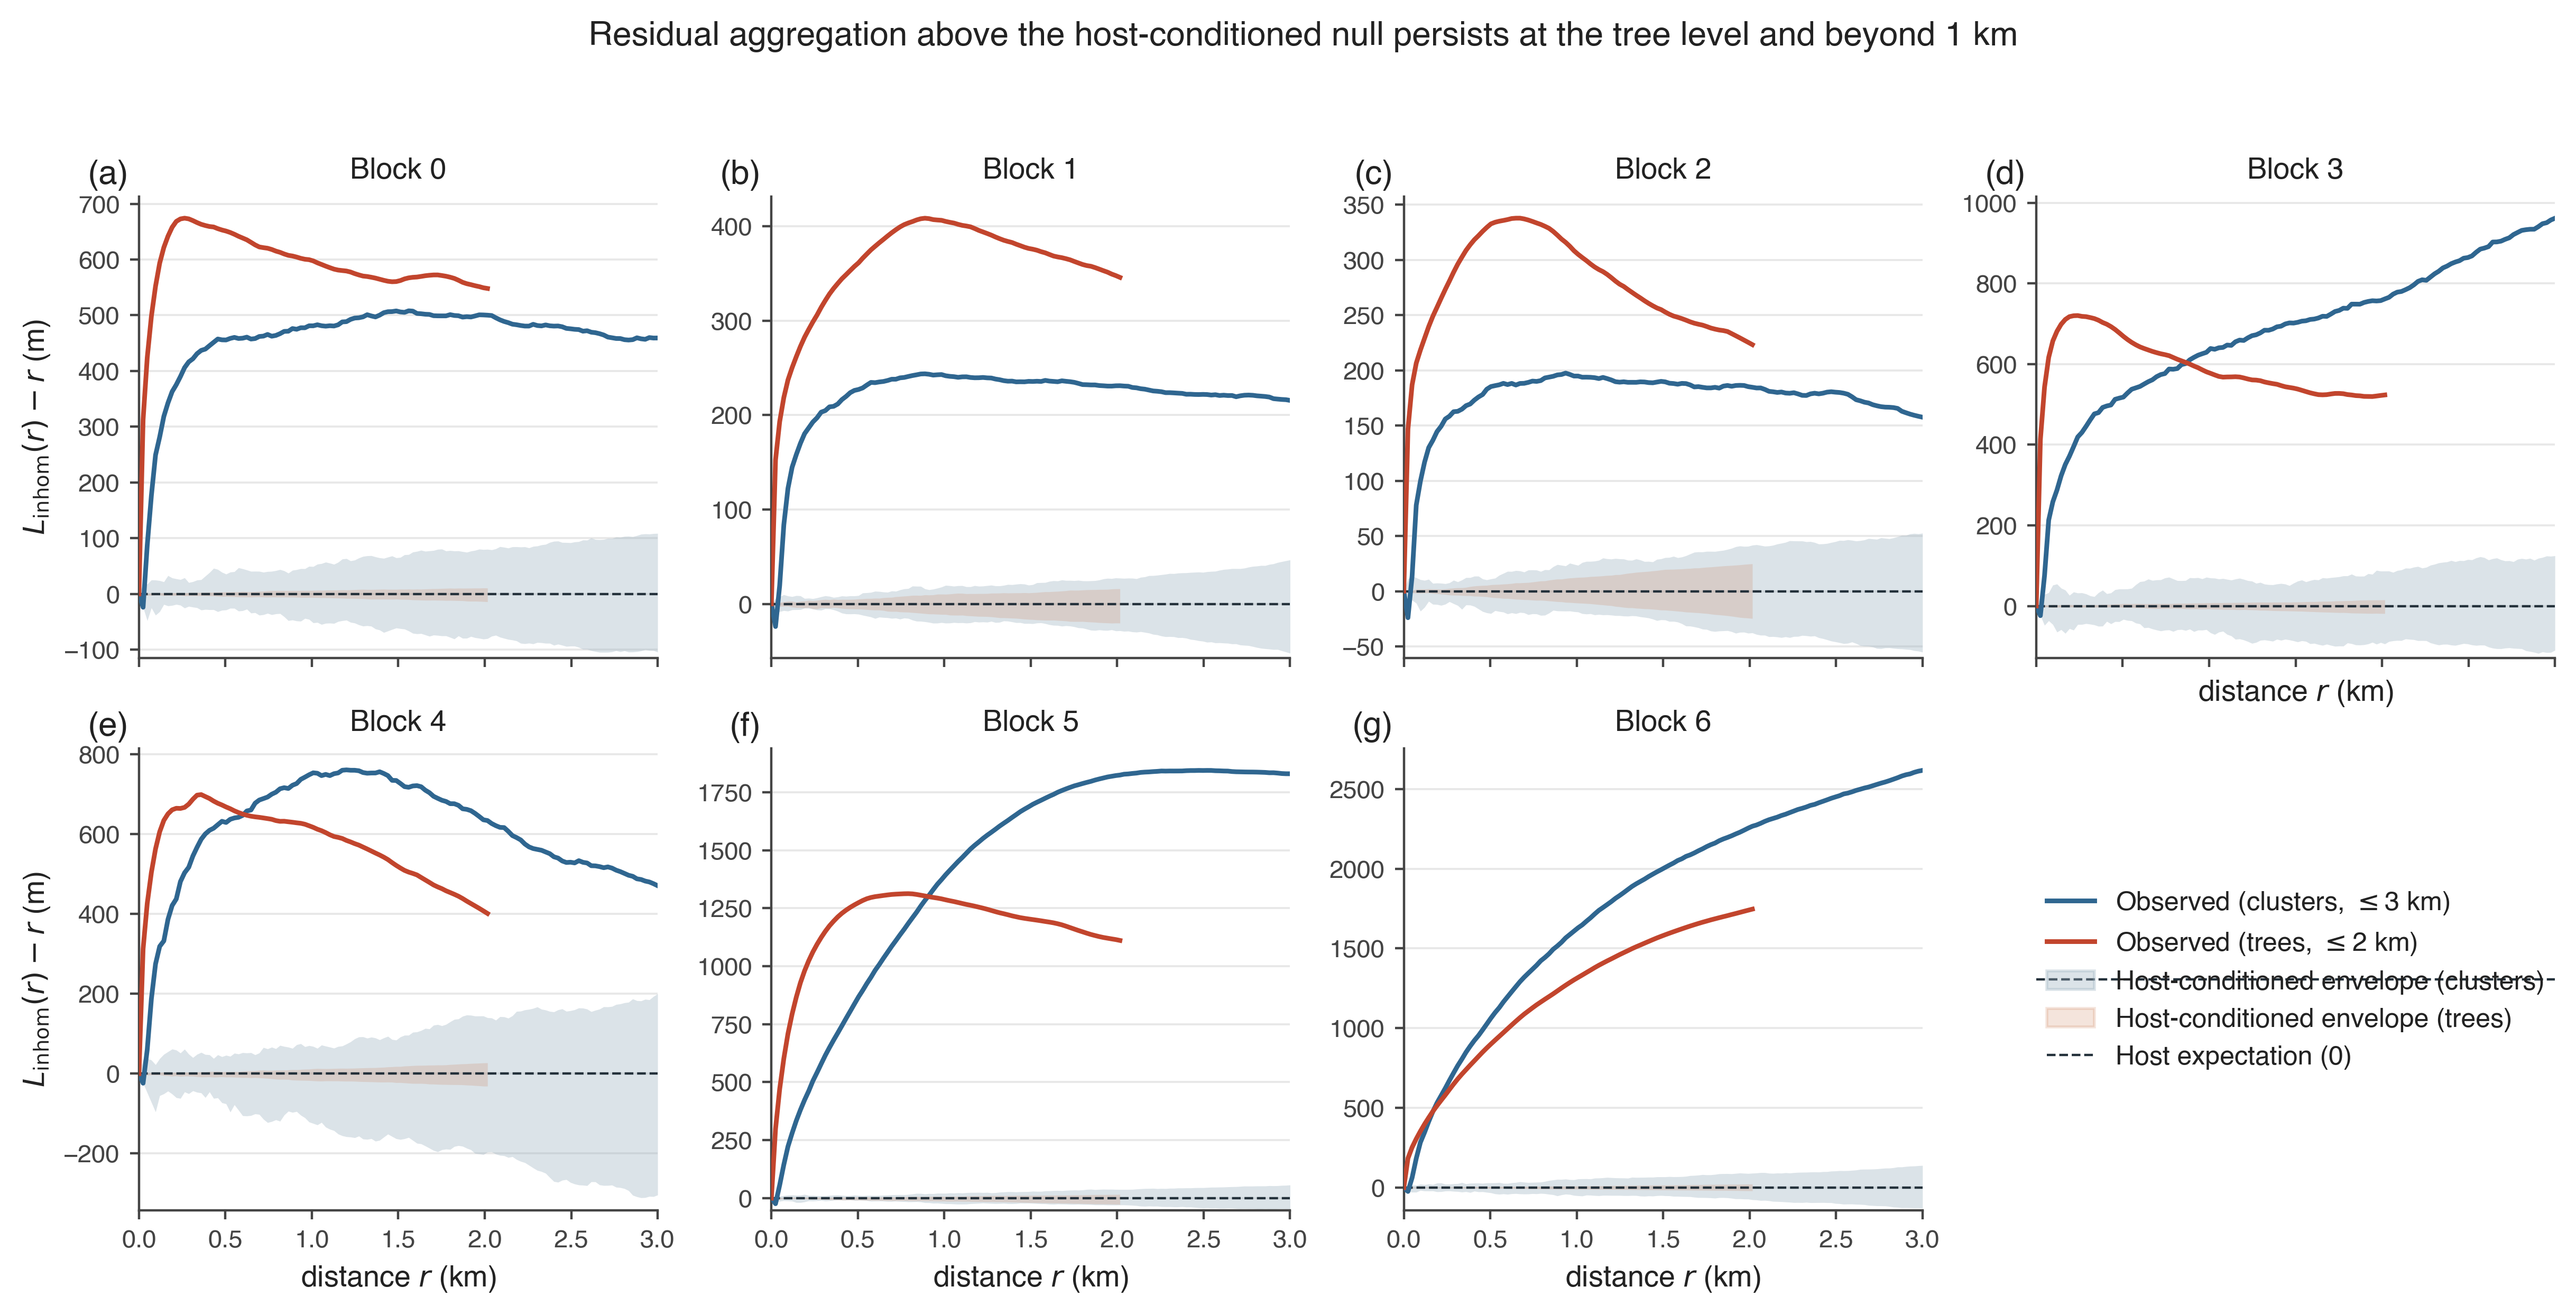
\includegraphics[width=\linewidth]{fig_hostcond_rigor.png}
  \caption{The residual aggregation is robust to the analysis unit and extends beyond 1\,km. Per-block
           $L_{\rm inhom}(r)-r$ for cluster centroids (blue, to 3\,km) and individual dead trees (red,
           to 2\,km), each against its own host-conditioned simulation envelope (shaded bands); the
           dashed line at $0$ is the host-conditioned expectation. In all seven blocks both observed
           curves lie above their envelopes across the whole range, so the local-contagion signal is
           not an artefact of using cluster centroids and is not confined to the sub-kilometre scale.}
  \label{fig:hostcond-rigor}
\end{figure}

\begin{figure}[htb]
  \centering
  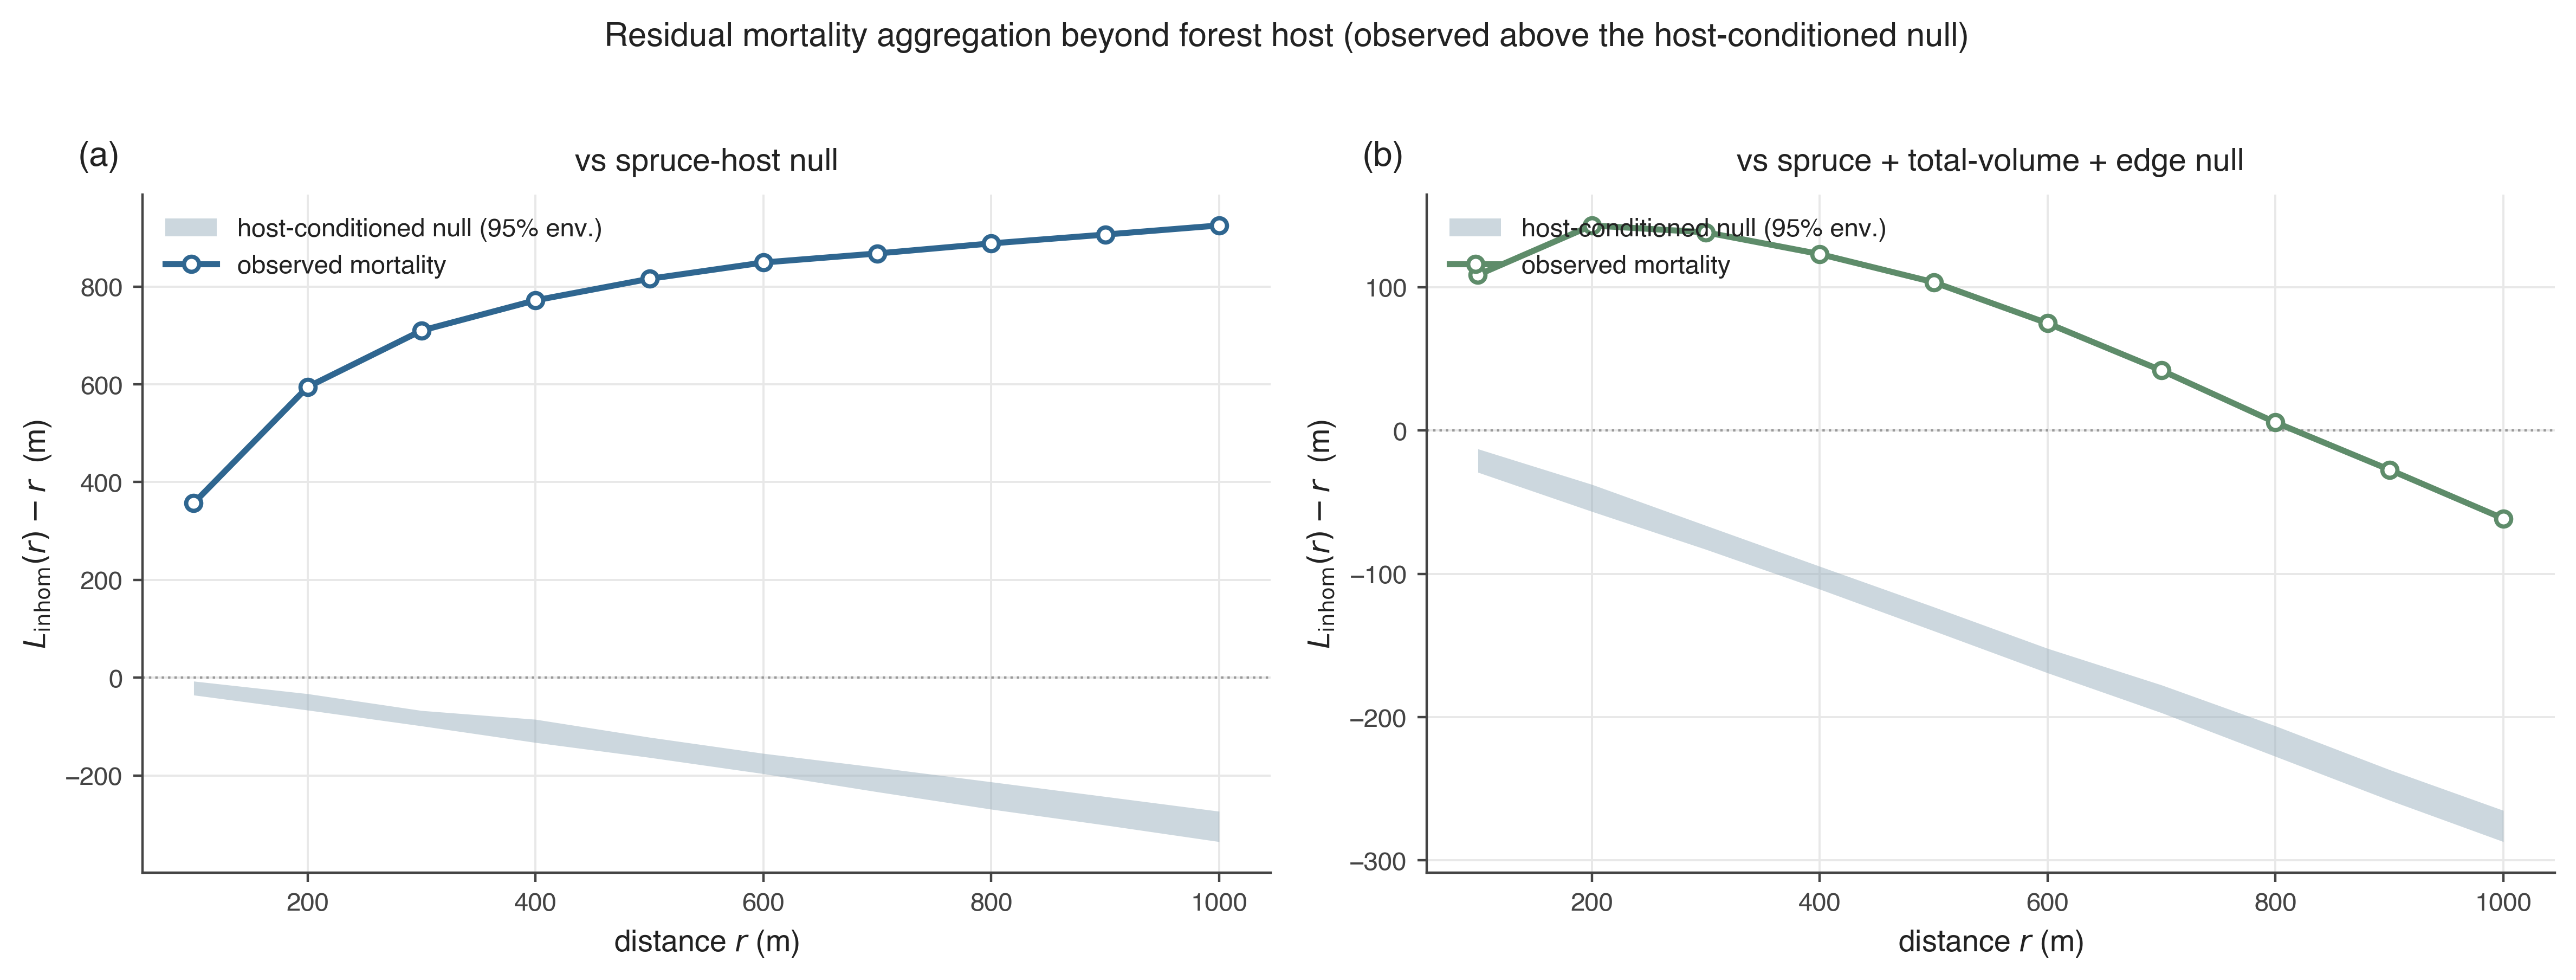
\includegraphics[width=\linewidth]{fig_host_conditioned.png}
  \caption{Residual mortality aggregation beyond forest host. Inhomogeneous $L_{\rm inhom}(r)-r$
           (observed, line) vs the host-conditioned 95\% simulation envelope (band).
           \textbf{(a)} spruce-only host null; \textbf{(b)} richer null (spruce\,+\,total
           volume\,+\,stand edge). Observed lies above the envelope across 100\,m--1\,km in both,
           so the residual sub-km aggregation survives the richer host model (its magnitude shrinks
           as total volume absorbs broader host structure). This tile-pooled ring estimator is valid
           to $r\lesssim1$\,km for the 6\,km tile windows; the larger-window \texttt{spatstat}
           estimator (Figure~\ref{fig:hostcond-rigor}) extends the range to
           3\,km.}
  \label{fig:hostcond}
\end{figure}

% ─────────────────────────────────────────────────────────────────────────────
\section{Discussion}
\label{sec:discussion}
% ─────────────────────────────────────────────────────────────────────────────

\mypar{What controls where dead trees concentrate?}
The central result is the host-conditioned one (Section~\ref{sec:res-host}): boreal canopy mortality
strongly tracks forest host availability (intensity rises with both spruce and total growing-stock
volume) yet retains a modest, genuine residual aggregation, robust to the analysis unit (cluster or
individual tree) and persisting from the sub-kilometre scale out to at least 3\,km, that survives
a richer host-conditioned null. Ecologically this is the signature of a process that is
\emph{first} constrained by where susceptible host stands are, and \emph{then} concentrates into
local foci within them rather than spreading diffusely, consistent with, though not proof of,
short-range contagion (bark-beetle tree-to-tree spread, or locally correlated wind/snow damage). The
honest weight of the claim is set by what conditioning removed: adding total volume to the null
absorbed most of the apparent excess, so the defensible statement is a \emph{bounded} residual, not
the order-of-magnitude clustering a naive (homogeneous-null) reading suggested.
This is also why we condition on a pre-mortality host and report structure rather than agents: the
same morphology arises from different agents (below), so the population-level second-order signal,
not patch shape, is what the data can support.

\mypar{Why don't patch shapes sort into distinct disturbance types?}
It is tempting to map the two endpoints onto dominant Finnish disturbance agents, the elongated,
internally dispersed Type\,0 onto wind-felled strips~\citep{gardiner2013wind, gregow2011combined},
and the compact, denser Type\,1 onto radially spreading beetle kill
\citep{raffa2008cross, jonsson2012epidemics, kautz2011simulating}. We deliberately resist this
mapping, because the evidence that would license it is either absent or circular. The shape-space
``reference zones'' are author-defined boxes in a space whose axes (aspect ratio, and the
compactness coupled to it) \emph{define} the gradient, so their overlap with the endpoints is a
restatement of the clustering, not external corroboration. Several confounders independently block
attribution: the detections themselves carry no species label, so a beetle-killed spruce cannot be
distinguished from a drought- or pathogen-killed pine, nor a compact patch from fire, snow-load,
or small salvage/clearcut polygons; the \texttt{alku\_aika} field records flight-strip
acquisition time, not mortality date, severing any link to specific storms or outbreak years; and
the single 2023 snapshot cannot separate a recent event from a years-old palimpsest of snags.
A compact morphology, in particular, is the default shape of almost any small mortality patch and
is therefore the least diagnostic possible signal, making a 76.5\% ``compact'' prevalence
uninformative about agent identity.

\mypar{External corroboration: morphology does not track species composition.}
The sharpest test of the circularity is to bring in a variable from outside the shape space and the
detector altogether. We attached the pre-mortality (2021) MS-NFI species composition (spruce, pine
and birch growing-stock volume) to every cluster at its location and asked whether the morphological
gradient covaries with the species mix of the stand that died (Section~\ref{sec:methods-host}, G5).
It does not. Within each block the Spearman correlation between aspect ratio and species fraction is
negligible ($|\rho|\le0.05$ for spruce, pine and birch; Figure~\ref{fig:species}a), and the two
morphological endpoints sit in near-identical species mixes (median elongated-minus-compact
difference $\le2$ percentage points for every species, with no consistent sign across blocks;
Figure~\ref{fig:species}b). The only relationships whose sign is reproducible across all seven
blocks, a faint tendency for more elongated patches to fall in slightly more broadleaf-rich, less
coniferous stands (birch $\rho=+0.05$, conifer $\rho=-0.04$, sign-test $p=0.016$), are an order of
magnitude too small to carry ecological, let alone agent-level, meaning. An external, non-shape
variable thus confirms what the internal diagnostics imply: patch morphology is not a proxy for
forest composition, so it cannot be read as a proxy for the agent that a given composition would
favour. This is the conservative outcome, and it strengthens the decision to withhold attribution.

\begin{figure}[htb]
  \centering
  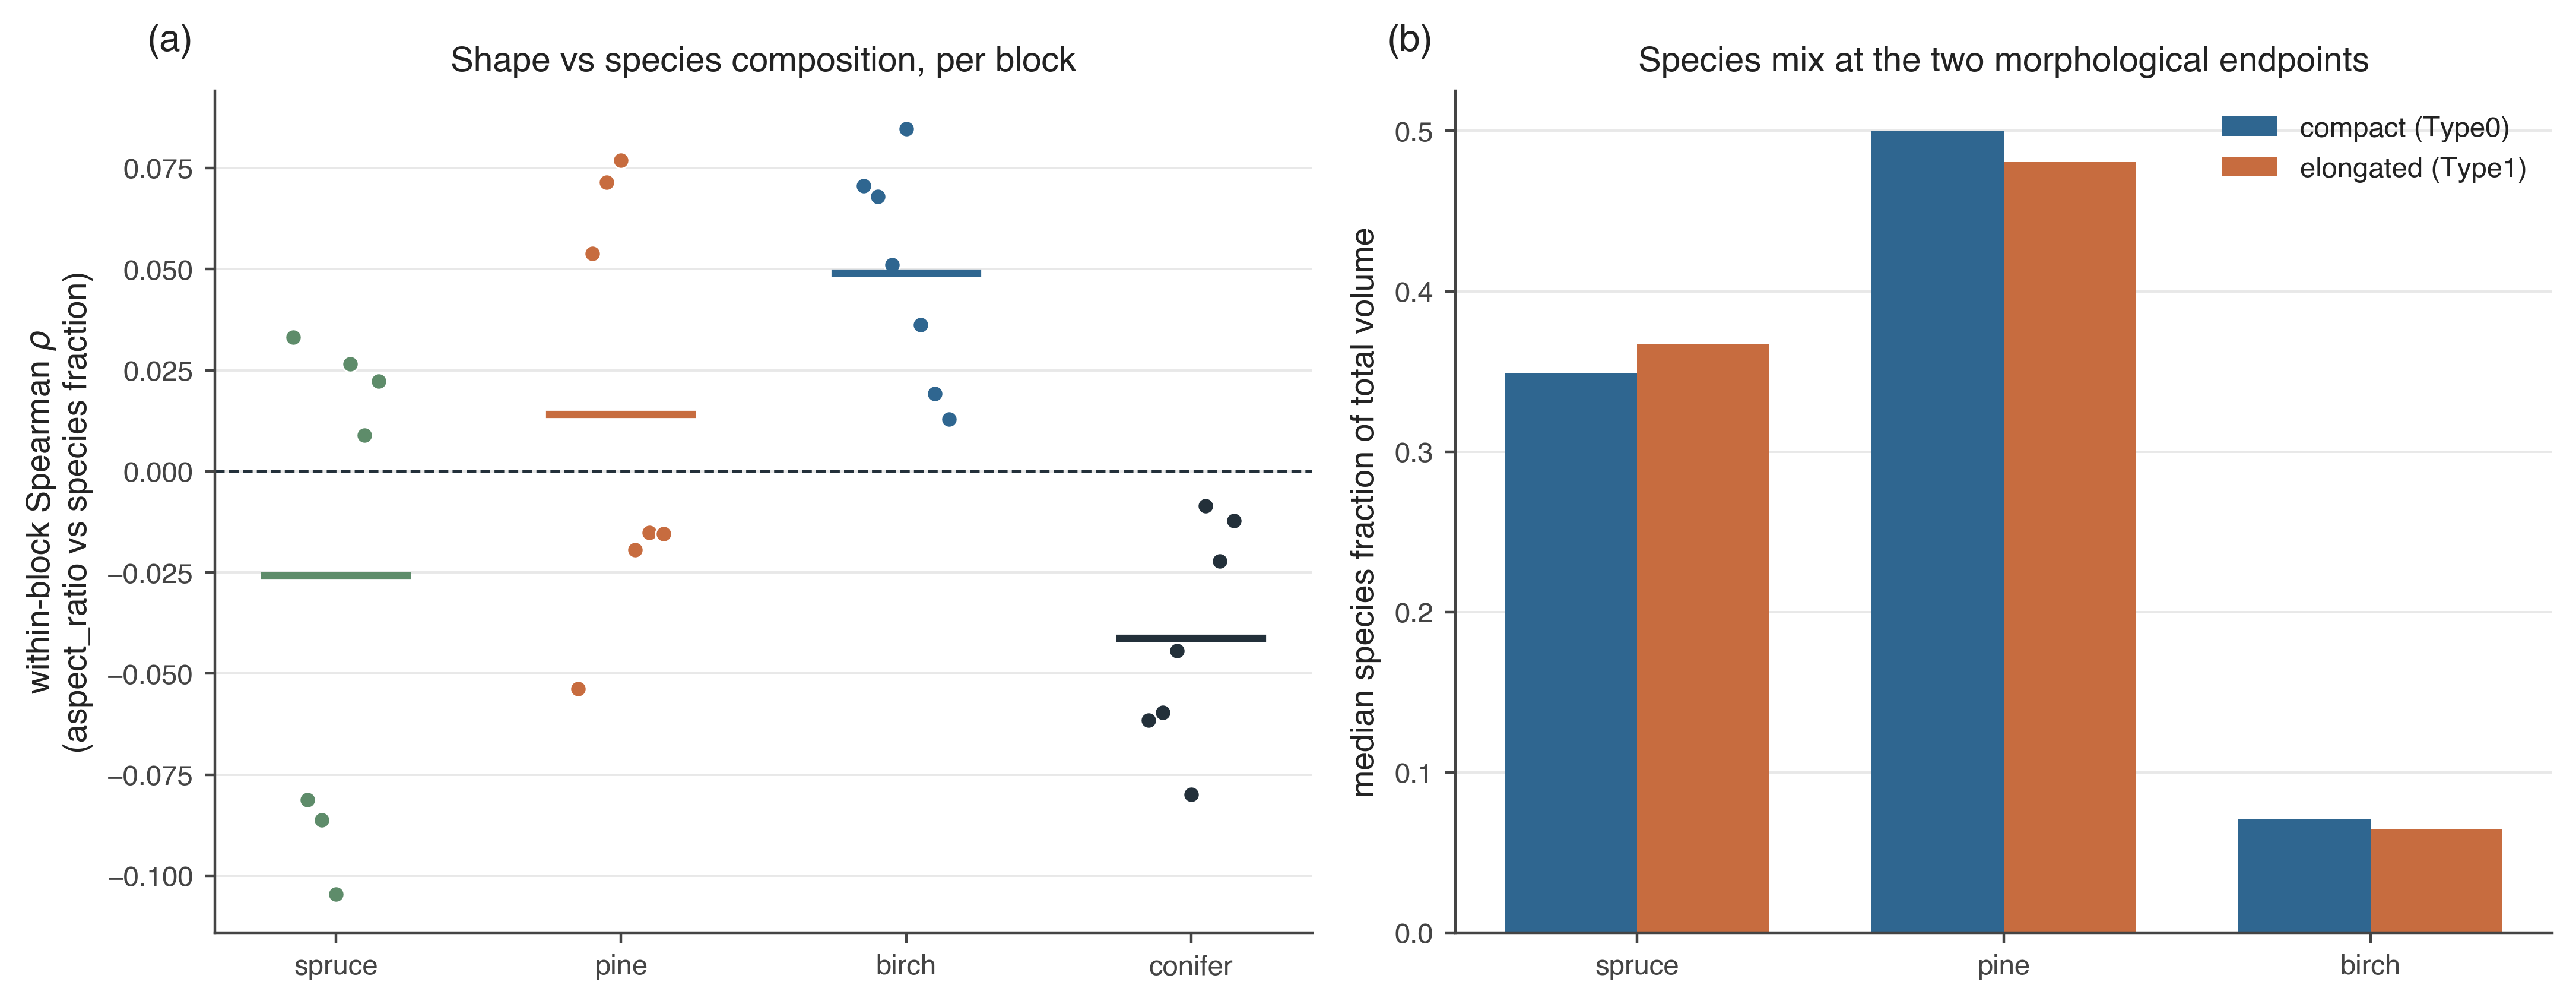
\includegraphics[width=\linewidth]{fig_species_validation.png}
  \caption{External validation against pre-mortality MS-NFI species composition (outside the shape
           space and the detector). \textbf{(a)} Within-block Spearman $\rho$ between cluster aspect
           ratio and the spruce/pine/birch/conifer fraction of stand volume; points are the seven
           blocks, bars the across-block means. All $|\rho|\le0.10$ and means near zero: the
           morphological gradient does not track species mix (the reproducible-sign but negligible
           birch$+$/conifer$-$ tendency aside). \textbf{(b)} Median species fraction at the compact
           and elongated endpoints is near-identical. Shape is not a proxy for forest composition.}
  \label{fig:species}
\end{figure}

\mypar{Do our own analyses point to a disturbance agent, or to geometry?}
\label{sec:disc-orientation}
The most telling evidence is internal and convergent. (i) \emph{Orientation.} The elongated
endpoint shows no preferred orientation ($r = 0.009$, $p = 0.747$), yet directional alignment
with storm tracks is the single most diagnostic fingerprint of windthrow. An elongated class with
no net direction is precisely what one would \emph{not} expect from wind, and it is the main
reason we decline the ``wind-thrown'' label. (ii) \emph{Scale dependence.} The prevalence of the
elongated endpoint moves with the DBSCAN radius (22.9\% at 40\,m to 28.6\% at 10\,m); a genuine
ecological class should be eps-stable, whereas a chaining artefact rescales with eps. (iii)
\emph{Connectivity.} The only shape-orthogonal feature, 200\,m reach, carries essentially no
discriminative signal (SHAP 0.005, last of seven). Read together, non-directional elongation,
eps-dependent prevalence, and no independent connectivity signal, the most parsimonious account
is that the typology summarises a continuum of \emph{detection-and-clustering geometry} (how dead-
tree detections chain together at a 20\,m radius, with mean within-cluster spacing of only
7.79\,m), rather than two distinct disturbance processes. The earlier ecological reading of the
size-frequency tails is correspondingly withdrawn: with the power law rejected in favour of a
lognormal for both endpoints, the heavier Type\,1 tail is explained by its larger mean area, not
by contagious spread.

\mypar{What does the held-out classifier's high accuracy actually mean?}
The AUC\,=\,0.976 shows that the two endpoints occupy largely non-overlapping regions of the
held-out feature space, but the SHAP decomposition shows why this is not independent validation:
performance is driven almost entirely by compactness and core-to-edge ratio, both geometrically
correlated with aspect ratio (a K-means input). The weakest predictor, reach\_200m
(SHAP\,=\,0.005), is the only feature capturing landscape connectivity independently of cluster
shape; its near-zero importance means the high AUC restates the K-means boundary through
correlated geometry rather than confirming it from new information. The honest reading is the
negative one: on the single axis genuinely independent of shape, the two endpoints are not
distinguishable.

\mypar{Limitations.}
Beyond the attribution caveats above, several additional limitations merit note. The upstream
deep-learning detection model is reported here without validation metrics (precision, recall), and
gate G4 shows its confidence score alone predicts type at AUC\,=\,0.727, so detection error,
likely structured by forest type, canopy density, and flight-strip geometry, is partly entangled
with the morphology we measure. Fully separating the two requires stratified detection
precision/recall against ground truth, which the present data lack; this is the single most
important outstanding check, and the Clark--Evans index, computed on a median of eight points per
cluster, is especially sensitive to it. The dataset is a national-scale but spatially
discontinuous sample (312 aerial tiles across Finland, in discrete latitudinal bands), so reported
prevalences are sample statistics rather than an exhaustive national census. Gate G1 confirms that the
eps\,=\,20\,m clustering scale partly determines the elongation it then measures. Finally,
because standing dead trees persist for years in boreal stands, a single-year snapshot cannot
date mortality: what we treat as one ``cluster'' may aggregate trees killed by different agents in
different years that happen to be co-located, so the unit of analysis is itself only loosely
defined, a fundamental limit on any morphology-to-process inference from one acquisition. Finally,
the 312 tiles form a purposive two-stage cluster sample (7 super-site blocks), not a probability
sample of the boreal zone, and the design is latitudinally imbalanced: 5 of the 7 blocks are
southern (60--62\textdegree{}N), while the central (65\textdegree{}N) and Lapland
(67.6\textdegree{}N) regimes are each represented by a \emph{single, unreplicated} block. Any
north--south contrast is therefore confounded with block identity: there is no way to separate a
latitude effect from one block's idiosyncrasy with $n=1$ block per northern regime. Findings
generalise to the within-landscape morphology of detected mortality at the southern super-sites
(where blocks are replicated); extension to central and northern Finland is provisional, and the
pooled gradient is a cross-regime description rather than a within-region or national estimate.
We did, however, verify that the gradient \emph{form} is reproduced within every block
(Table~\ref{tab:blocks}), so the principal result does not depend on the relative weighting of
regions; what the design cannot support is any claim about the national frequency or distribution
of mortality morphologies.

\mypar{Future work.}
Several steps would extend the host-conditioned result, in increasing order of data requirement.
The two pure-computation refinements that the analysis itself called for, a tree-level (rather than
centroid) treatment of the inhomogeneous point process and a variance-stabilised, large-window
estimator reaching reliably past 1\,km, are carried out here (Figure~\ref{fig:hostcond-rigor});
both confirm the residual aggregation. The remaining steps need new layers. First,
with publicly available layers: overlaying a species layer from Finland's multi-source national
forest inventory and a regional disturbance-agent map (e.g.\ Metsäkeskus damage records) would
enable a marked point-process test, moving from \emph{characterising} spatial structure to
\emph{attributing} it; we note that the pan-European attribution products
\citep{senf2021mapping} group wind and bark beetle into a single class and so cannot, by themselves,
separate the two agents, which is why a dedicated regional layer is required. A complementary
detection-validation step (stratified precision/recall against field or photo-interpreted ground
truth) would calibrate, rather than merely bound, the detector confound. Second, and requiring new
acquisition rather than further analysis of the present data, multi-temporal imagery (prior-year
aerial surveys passed through the same detector, which are not available for this study) would add
the temporal dimension: it would date mortality, separate recent deaths from years-old snags, and
turn the static host-conditioned pattern into a space-time process, the definitive test of whether
this year's foci predict next year's mortality. The pipeline itself is computationally scalable and,
once these layers are in place, could support comparative analysis across the Nordic countries.

% ─────────────────────────────────────────────────────────────────────────────
\section{Conclusion}
\label{sec:conclusion}
% ─────────────────────────────────────────────────────────────────────────────

We have analysed 698,223 individual dead-tree detections from a 2023 national-scale aerial sample
(seven boreal super-sites, southern boreal zone to Lapland) as a host-conditioned point process.
Conditioning on a pre-mortality forest-inventory host surface, we find that canopy mortality
strongly tracks forest host availability (intensity rises with spruce and total growing-stock
volume) and yet retains a modest, genuine residual aggregation at the sub-kilometre scale that
survives a richer host-conditioned null, a local-contagion signature on top of host-tracking,
established with inhomogeneous second-order statistics and host-conditioned simulation envelopes.
We deliberately report this spatial \emph{structure} rather than disturbance-agent labels, because a
candidate morphological ``typology'' of the clusters does not survive scrutiny. Using DBSCAN
clustering, Donnelly-corrected Clark--Evans statistics, and a suite of complementary shape metrics,
the morphology of detected mortality clusters is organised by a dominant
compactness--elongation gradient. This gradient is not a statistical artefact of correlated
features: the $k=2$ silhouette (0.401) exceeds a covariance-preserving null at $p = 0.001$. The
\emph{discrete} two-class reading of that gradient, however, does not survive scrutiny. Mixture-model
selection and the unimodality of the dominant axis already indicate a continuum rather than two
modes; four stability gates confirm it. Re-clustering from raw, the partition is not invariant to
the DBSCAN radius (G1), its 23.5\%/76.5\% split is an artefact of the aspect-ratio filter and
dissolves into a single continuous tail once that filter is released (G2), the elongated class
carries no directional structure beyond hull shape (G3, consistent with the orientation null), and
it is partly predictable from detector confidence alone (G4). The held-out Random Forest
(AUC\,=\,0.976) reproduces the split only through geometric redundancy among shape descriptors, the
one shape-orthogonal feature, landscape connectivity, adds no signal.

The framework demonstrates that remote-sensing-derived maps of dead-tree locations contain a
recoverable and reproducible morphological gradient, but that the temptation to discretise it into
disturbance types must be resisted on the present evidence. The discrete partition is an artefact of
clustering scale and a filter applied to its own defining axis, with no second-order content and a
measurable detector confound; the gradient is what is real. Rather than a ready ``first filter'' for
the field, the pipeline is best positioned as a hypothesis-generating characterisation whose
ecological meaning must be established by overlay with independent disturbance-agent maps, species
layers, and multi-temporal imagery, a programme we outline as the natural next step.

% ─────────────────────────────────────────────────────────────────────────────
\section*{Data and Code Availability}
The dead-tree detections analysed here were produced by the U-Net segmentation model of
\citet{junttila2024significant} applied to 2023 National Land Survey of Finland aerial imagery; the
derived cluster-level table (14,582 clusters with shape, point-pattern, and connectivity metrics) and
the per-tree coordinates are released with the analysis code. The host and species covariates are the
public multi-source national forest inventory (MS-NFI / MVMI) growing-stock volume and land-class
rasters of the Natural Resources Institute Finland (Luke; CC-BY 4.0, 16\,m, EPSG:3067), pre-mortality
(2021) vintage: \texttt{kuusi} (spruce), \texttt{manty} (pine), \texttt{koivu} (birch),
\texttt{tilavuus} (total volume) and \texttt{maaluokka} (land class), file stamp \texttt{vmi1x\_1721},
retrieved from the Paituli / funet geodata archive
(\texttt{rsync.nic.funet.fi/index/geodata/luke/vmi/2021/}). All analysis code (clustering, shape
metrics, the four falsification gates, the host-conditioned point-process engine and its
\texttt{spatstat} cross-check, and the external species validation) is available at
\url{https://github.com/aniskhan25/TreeMortSpatial}. The national raster tiles are redistributed by
Luke and are not duplicated in the repository; the \texttt{rsync} paths above reproduce them exactly.

\section*{Reproducibility}
Analyses were run with Python 3.9.6 (numpy 2.0.2, scipy 1.13.1, pandas 2.3.3, scikit-learn 1.6.1,
geopandas 1.0.1, rasterio 1.4.3, shapely 2.0.7, pyproj 3.6.1, pointpats 2.3.0, matplotlib 3.9.4) and
R 4.6.1 with \texttt{spatstat} 3.6.1. All stochastic steps are seeded: the covariance-preserving null
and discreteness tests use seed 42, the per-block tree subsampling for the tree-level point process
uses seed 42, and the \texttt{spatstat} envelopes use 39 host-conditioned simulations per block
(self-tested on inhomogeneous-Poisson patterns). DBSCAN (\texttt{eps}\,=\,20\,m for clusters,
15\,km for blocks; \texttt{min\_samples}\,=\,1 for the block grouping) is deterministic. Software
versions, per-figure provenance, the shape-feature correlation matrix, and univariate feature AUCs
are tabulated in the Supplementary Information.

% ─────────────────────────────────────────────────────────────────────────────
\bibliographystyle{unsrtnat}
\bibliography{sample-base}

\end{document}
